\documentclass[authoryearcitations,11pt]{UoYCSproject}

\setcounter{tocdepth}{1}
\title{Implementing Test Coverage in Epsilon}
\author{Thomas Wormald}

\date{\today}
\SWE
\supervisor{Dr. Louis M. Rose}
\abstract{Testing is absolutely critical on any piece of software, but being sure that the tests are comprehensive is not easy. Test coverage is one way of increasing confidence in a test suite by monitoring which statements, branches, paths etc. have been executed to ensure that no parts of the code have been missed by the test suite.

In this project I have developed a framework for measuring test coverage that is used to enhance EOL, a domain-specific language.

The framework that I have developed is extensible. When designing and implementing branch coverage I opted to convert the Abstract Syntax Tree (AST) to a Control Flow Graph (CFG) because this will make path analysis a lot easier to implement in a future project, and may also be useful for other types of program analysis. The conversion proved to be challenging because there is no in depth documentation of the algorithm. I therefore had to perform analysis for each type of statement, and justify any design deicions that were made.

The framework was evaluated by application of a case study on a large EOL program (EuGENia). The study showed that there were significant gaps in the test coverage of EuGENia, which can now be addressed by the Epsilon developers.}
%\dedication{Dedication: To be decided}
%\acknowledgements{I would like to acknowledge that this dissertation would probably be a lot better without Tommy Fong, whose nighclub The Willow provided far too many cheap drinks that have rotted my brain over the last 4 years.}
\wordcount{24197}
\begin{document}
\maketitle
%\listoffigures
%\listoftables
%\renewcommand*{\lstlistlistingname}{List of Listings}
%\lstlistoflistings
%\doublespacing

%\cleardoublepage
%\part{Preliminaries}
%\label{sec:start}
%\thispagestyle{empty}\cleardoublepage

%\setcounter{page}{1}

\chapter{Introduction}

Welcome to the best project write-up ever.

\chapter{Literature Review}

\section{Introduction}
% This introduction is pretty poor, probably best to rewrite once the rest is finished
In this chapter I will give an overview of the existing literature that is appropriate to my project. The chapter is split into two sections. The first section gives a review of Model Driven Engineering and tools that can be used for implementation. The second section investigates software testing methods and ways of assessing the quality of software tests.

\section{Model Driven Engineering}

\subsection{Introduction}
% The Oxford English dictionary defines Model Driven Engineering as... just kidding
Model Driven Engineering is a development methodology that aims to reduce the amount of time spent on projects, as well as increasing the consistency and quality of the item or system under development. One example of when model driven engineering is useful is when developing applications. A model of the system can be developed. This model can then be converted into code. Assuming that the model is correct, human typing errors are avoided and precious development time can be spent on more important aspects that hunting for trivial bugs. Maintenance is also easier, as changes can be applied to the model, and the updated code will be generated automatically from the model. Finally, the code generation can be to a multitude of languages and platforms, further reducing time spent on development \cite{mdseLano}.

%Model Driven Engineering is a development methodology that aims to reduce the amount of time spent on code development by building models that can be transformed and used to generate code automatically. Bugs that would normally be in code (through developer error) will no longer be present, as all the code has been generated automatically from a model. Of course this assumes that the model is correct in the first place. Cross-platform implementation overheads are also reduced. The model can remain the same for all platforms, and only the model-to-code program has to be modified for different target platforms. \citep{mdseLano}.

In the 1980's there was a software quality crisis that lead to the search for alternative approaches to developing software. Model Driven Engineering is one solution that was of interest at the time as it provided a way to visually represent a system architecture, and from that generate code automatically. However, the return on investment that companies were expecting from model driven engineering was far too high, causing much disappointment and disillusionment, and for a while the concept was sidelined. More recently, the Object Managment Group (OMG) have promoted and developed a Unified Modeling Language (UML), and tools such as Epsilon have further promoted the use of MDE \citep{mdeHistory}.  \citet{brambillaBook} believes that Model Driven Engineering is now past the `trough of disillusionment' and into the `slope of enlightenment' (see figure \ref{mde_pos}) \\

\begin{figure}
\begin{center}
	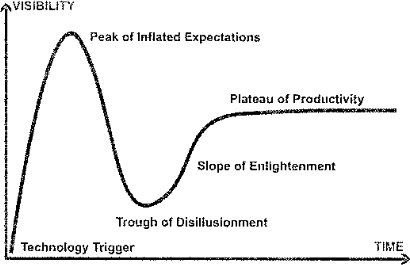
\includegraphics[width=4in]{figures/mde_pos.jpg}
\end{center}
\caption{The technology hype cycle according to \citet{brambillaBook}}
\label{mde_pos}
\end{figure}

\subsection{Model}

\begin{figure}
\begin{center}
	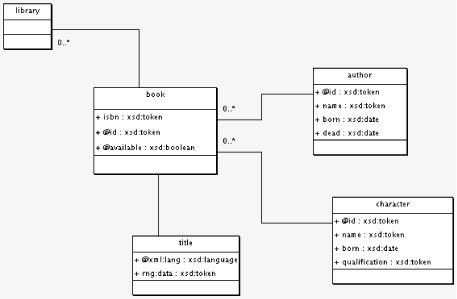
\includegraphics[width=4in]{figures/sample_model.jpg}
\end{center}
\caption{A sample model}
%TODO: Create my own model to sample here?
\label{uml_sample}
\end{figure}

A model is a representation of something that abstracts away many details that are not necessary for its use \citep{brambillaBook}. For example, the Utah Teapot \citep{utahTeapot} is a model of a teapot that is rendered by a 3D engine. However, many aspects of the teapot are not considered in its model, as they are not necessary for a simple render. An example is that the lid is not a removable component, because for the purpose of rendering the teapot, the lid never has to be removed. Another example is that the only physical property of the teapot that will be included in the model is it's finish (texture), so that lighting and reflection can be calculated. Other details such as its weight will not be included in the model, because it isnot necessary.

UML (Unified Modeling Language) is a language that is designed specifically for representing models visually. It is ideal for object-oriented design, as it represents classes with boxes and links between classes with lines. Within the boxes there are definitions of the classes (spelling?) methods and fields. In figure \ref{uml_sample}, author is a class that has properties such as name, born, dead. The diagram also shows that there is a connection between author and book.
%TODO: Write about the connection, or update to a better sample model

\subsection{Metamodels}
To have a modeling language, there must be a specification of that language that defines the valid syntax, constraints etc. In the case of UML, the Object Management Group provide a detailed specification \citep{umlSpec} of the language, and we can check that any diagram is a UML diagram by checking it against the UML specification.
%Concrete, Abstract and semantic sections...
A metamodel is the specification of a modeling language, in the form of a model \citep{brambillaBook}. A metamodel could be represented visually or textually, depending on the specification of the metamodeling language. As with many aspects of computer science, the metamodel is just another layer of abstraction, and we can continue to abstract to higher and higher levels. A metametamodel (known as M3) will define the specification of a metamodeling language, and the abstraction can continue as far as is required.

Going back to the example of The Utah Teapot, the metamodel in this case may define that the teapot is made up from interconnected polygons, and specify that each polygon has a location and size given in 3D space. 

\subsubsection{Abstract and Concrete Syntax}

When building a metamodel, both the abstract and concrete syntax must be defined. The abstract syntax of a language is a definition of how the language components interact. For an OO language, the abstract synatax would specify that a class can inherit the properties of another class, that a class must have a constructor, and that a class must be given a name. How these requirements are met by the user is specified by the concrete syntax. The concrete syntax for allowing class inheritance would state that the colon symbol must be used after the class name:

\begin{lstlisting}
class NewClass : ParentClass
\end{lstlisting}

The concrete syntax does not necessarily need to be textual. To build a modeling language you require a metamodel, which is the abstract syntax. You also require a way to visually display the model. The concrete syntax could state that a class is represented as a rectangle with the name of the class in the middle, and that to show inheritence the NewClass must have an arrow coming out of it that goes to the ParentClass that it is inheriting from.

\begin{figure}[h]
\begin{center}
	
\includegraphics[width=2in]{figures/concrete_syntax.png}
	\label{concreteSyntaxFigure}
	\caption{Concrete Syntax example for a modeling language}
\end{center}
\end{figure}

\subsection{Graphical Modeling Framework}

The Eclipse graphical modeling framework (GMF) is part of the Eclipse Graphical Modeling Project \citep{gmpSite}. The Eclipse Wiki \cite{gmpFAQ} defines GMF as:

\begin{quote} Using GMF, you can produce graphical editors for Eclipse. For example, a UML modeling tool, workflow editor, etc. Basically, a graphical editing surface for any domain model in EMF you would like. \end{quote}



\subsection{Epsilon}
To be able to perform Model Driven Engineering, we of course require some tools and languages to build and manipulate models. These tools could be built from scratch for each project, but that would be a waste of time.

Epsilon is a suite of languages and tools that provide all the necessary components to build and manipulate models. Epsilon stands for \textbf{E}xtensible \textbf{P}latform of Integrated \textbf{L}anguages for M\textbf{O}del Ma\textbf{N}agement \citep{epsilonWebsite}. It is part of the Eclipse Modeling Project \citep{ecliplseModelingProjectSite}, and includes tools for each of its languages that integrate with Eclipse. From the Epsilon Website \citep{epsilonWebsite}, the languages that are provided by Epsilon are:

\begin{description}
\item[EOL] Epsilon Object Language is an expression language that is used to create, query and model EMF models.
\item[ETL] Epsilon Transformation Language is a model-to-model transformation language.
\item[EVL] Epsilon Validation Language is a model constraint language.
\item[EGL] Epsilon Generation Language is a model-to-text generation language that can be used to generate code from models.
\item[EWL] Epsilon Wizard Language is similar to ETL, except that ETL performs batch operations whereas EWL works with in-place model transformations based on user selections.
\item[ECL] Epsilon Comparison Language is a model comparison language.
\item[EML] Epsilon Merging Language is used to merge models of diverse metamodels.
\item[Epsilon Flock] A rule
\end{description}

Together these languages provide a powerful framework for model driven engineering.

\subsection{EuGENia}
EuGENia is one of the tools that is included with Epsilon. EuGENia takes an Ecore metamodel specification and generates a GMF editor \citep{eugeniaSite}. From the code in \ref{cha:EugSampCode}, the model editor shown in figure \ref{sampleGmf} is generated by EuGENia.

\begin{figure}
\begin{center}
	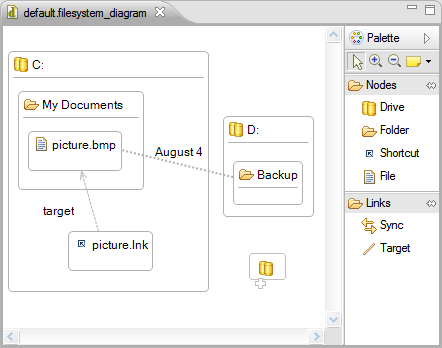
\includegraphics[width=4in]{figures/gmfeditor.png}
\end{center}
\caption{A sample gmf editor generated by EuGENia \citep{eugeniaSite}}
\label{sampleGmf}
\end{figure}

The generator editor provides the objects shown on the right hand side of figure \ref{sampleGmf}. These objects are then dragged to the left hand section of the editor by the user, where connections between objects can be intuitively created. 

\subsection{EuGENia Live}

EuGENia Live is a web-based version of EuGENia that removes some of the complexity of getting started with EuGENia. The EuGENia Live Paper \citep{eugeniaLivePaper} describes EuGENia Live as: \begin{quote}... a tool for designing graphical DSLs  \end{quote}

However, unlike EuGENia, EuGENia  Live is a visual tool that allows you to switch back and forth between graphical editing of a DSL and the code for the DSL. Figure \ref{eugeniaLiveGraphical} shows EuGENia Live graphically editing a DSL, and Figure \ref{eugeniaLiveCode} shows the same DSL's code being edited in EuGENia Live.

\begin{figure}[h]
\begin{center}
	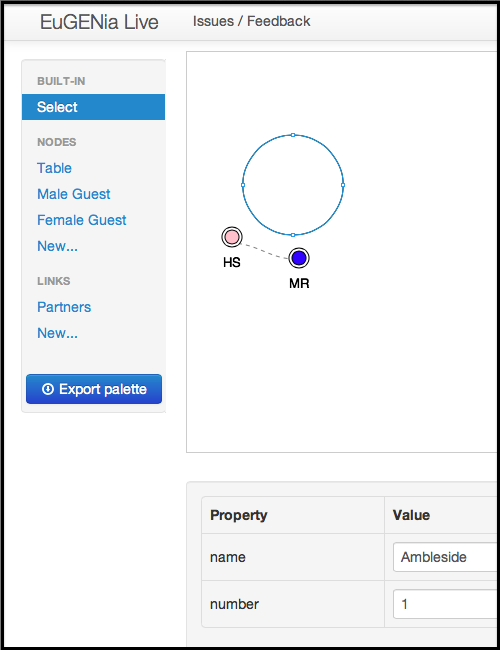
\includegraphics[width=4in]{figures/eugenia_live_graphical.png}
\end{center}
\caption{EuGENia Live's Graphical Editor \citep{eugeniaLiveDocumentation}}
\label{eugeniaLiveGraphcal}
\end{figure}

\begin{figure}[h]
\begin{center}
	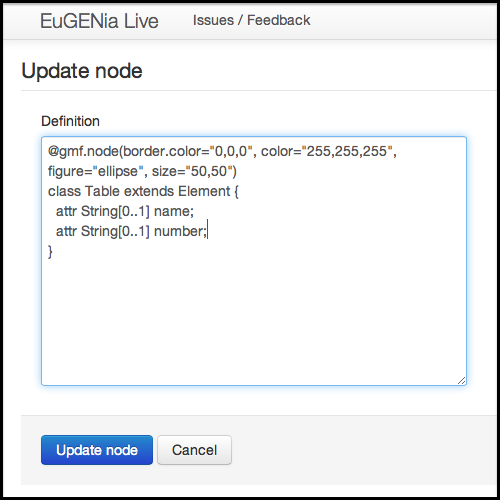
\includegraphics[width=4in]{figures/eugenia_live_code.png}
\end{center}
\caption{EuGENia Live's Code Editor \citep{eugeniaLiveDocumentation}}
\label{eugeniaLiveCode}
\end{figure}


\section{Quality of Software Testing}
\subsection{Introduction}
Software testing is a crucial part of the development cycle of any serious piece of software. Developers can make changes to code that make it do what they want, but could break another part of the program that uses the same code. Suites of tests can be implemented that \emph{should} notice if a developer breaks the code, but there is the possibility that the correct tests have not been implemented to catch a certain fault.

The Ariane 5 rocket cost \$7 billion to develop, and so of course any software on board would have had test suites to ensure that it did not fail. Unfortunately, 37 seconds after launch, \$500 million of rocket and cargo exploded because of an integer overflow \citep{ariane5}. Despite having software tests, the test `coverage' must have not been sufficient, leading to such a disaster. This is of course an extreme example, but it highlights the need for not only software testing, but good quality software testing.


% Section about testing requrements
\subsection{Coverage}

Test sets have a \emph{coverage criterion} that measures how good a collection of sets is \citep{softwareTestingIntro}. According to \citet{softwareTestingIntro}, coverage is defined as:

\begin{quote} Given a set of test requirements $TR$ for a coverage criterion $C$, a test set $T$ satisfies $C$ if and only if for every test requirement $tr$ in $TR$, at least one test $t$ in $T$ exists such that $t$ satisfies $tr$ \end{quote}

In addition to coverage, coverage level is also defined by \citep{softwareTestingIntro} as:

\begin{quote}Given a set of test requirements $TR$ and a test set $T$, the coverage level is simply the ratio of the number of test requirements satisfied by $T$ to the size of $TR$\end{quote}.

There are different approaches to determining the test coverage level of a program. Below I discuss each of these.

\subsection{Statement Coverage}

% ToDo: Find a source other than what Louis told me in lectures...

Arguably the simplest approach to determining the quality of a test set is to analyse the number of lines of code that execute when the tests are run. If all lines of code are executed at least once when all tests have been run, then statement coverage is said to be 100\% \citep{something}.

While simple to implement, line coverage suffers from an obvious downfall. In most programming languages it is perfectly valid to have as many operations on one line as the developer chooses. In an extreme case it would be possible for the developer to have the whole program on one line. A contrived example of this is shown in Figure \ref{lineCoverage}. If a test was created that executed that program, the coverage should come back as 100\%, regardless of whether the test tried to run the program with different date's set on the test machine or not.

\begin{figure}
	\begin{center}
		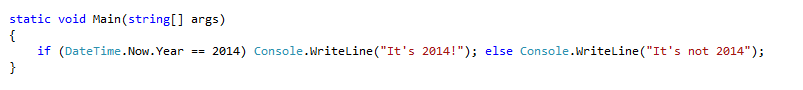
\includegraphics[width=6in]{figures/line_coverage.png}
	\end{center}
\caption{A valid program that is all on one line.}
\label{lineCoverage}
\end{figure}

An easy but non-ideal solution to this is to require that developers only place one statement on each line. Alternatively, a more complex coverage analysis tool could be used that takes this into account.

Statement coverage is the term used when talking about the number of program statements that are executed by testing \citep{Myers:2004:AST:983238}. \citet{Myers:2004:AST:983238} argue that statement coverage is `generally useless' as a metric of test quality because of the number of problems that it can potentially miss.

The example provided by \citet{Myers:2004:AST:983238} gives the code as shown in Figure \ref{codeCoverage}. They argue that a single test can provide 100\% statement coverage for the code by passing in the values \verb+A=2, B=0, X=3+, even though the code could be logically incorrect. The example that they provide is that if the first decision should be an \verb+or+ instead of an \verb+and+, then the single test will not notice, despite providing 100\% statement coverage.

\begin{figure}[h]
	\begin{center}
		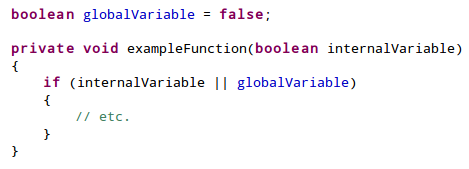
\includegraphics[width=2in]{figures/code_coverage.png}
	\end{center}
\caption{The sample code provided by \citet{Myers:2004:AST:983238}.}
\label{codeCoverage}
\end{figure}

\subsection{Branch Coverage}

\subsubsection{Control Flow Graph}

Before branch coverage can be introduced, the concept of a program control flow graph must be explained. A control flow graph shows the potential paths through a piece of code. Figure \ref{cfg} shows the control flow graph for the code listed in Figure \ref{codeCoverage}. At the top of the control flow graph is the entry point to the graph. From there, the first conditional statement is represented as a vertex of the graph. From that vertex there are two outward arrows. One represents the case when the conditional statement evaluates to true, and the other to false \citep{Myers:2004:AST:983238}

\begin{figure}
	\begin{center}
		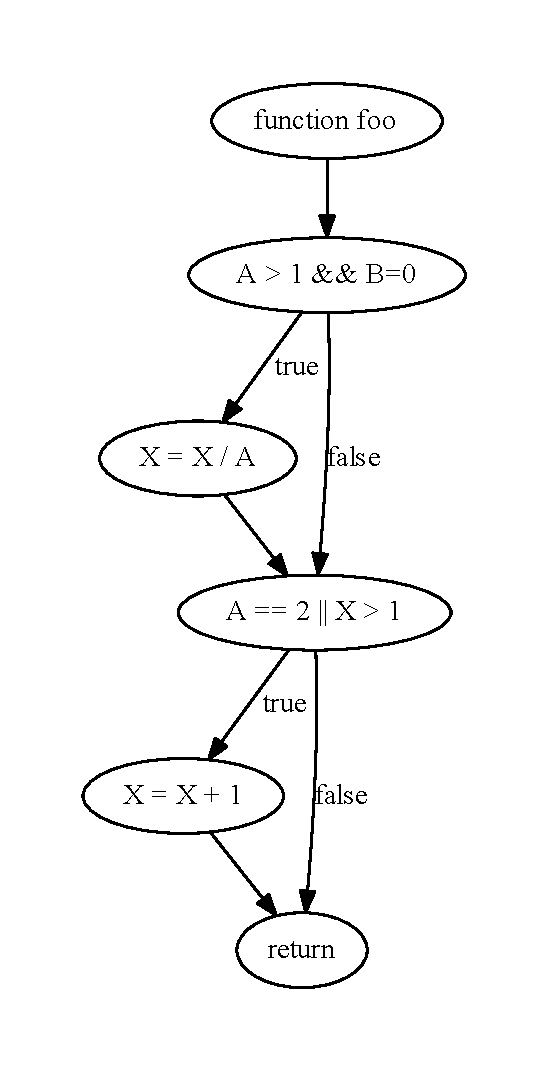
\includegraphics[scale=0.5]{figures/cfg.pdf}
	\end{center}
\caption{A simple control flow graph for the function foo}
\label{cfg}
\end{figure}

\subsubsection{Branch Coverage}

Branch coverage then is the number of branches that have been executed within the control flow graph. In Figure \ref{cfg} there are two branching points - both of the conditional statements. For 100\% branch coverage it is necessary for every edge to have been executed at least once by the test set. An alternative way to think of this is that at every decision point in the program, the outcome of each decision has been executed at least once. At an \verb+if+ statement, the case where the outcome is true has been executed as well as the case where the outcome is false. If branch coverage is 100\%, then so should statement coverage \citep{Myers:2004:AST:983238}.

However, \citet{Myers:2004:AST:983238} also argue that branch coverage can be a weak test quality metric. Going back to the code listed in Figure \ref{codeCoverage}, branch coverage can be satisfied with the two following test cases: \verb+A=2, B=0, X=1+ and \verb+A=3, B=1, X=1+. However, if the second conditional statement was supposed to check that X < 1 instead of X > 1, then this will not be picked up by any tests, despite the branch coverage being 100\%. \citet{497650} have done a comparison of the effectiveness of decision coverage (i.e. branch coverage) and block coverage (i.e. statement coverage) after they inserted some random faults in the Unix utility Grep. Their results show in Figure \ref{coverageReliability} that block coverage analysis requires a higher percentage of coverage to find the same number of faults when compared to decision coverage.

\begin{figure}
	\begin{center}
		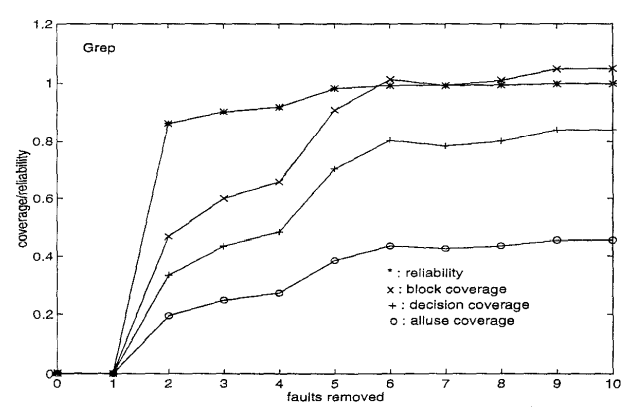
\includegraphics[width=5in]{figures/coverage_reliability.png}
	\end{center}
\caption{\citet{497650}'s results of testing various coverage approaches on Grep}
\label{coverageReliability}
\end{figure}

\subsection{Path Coverage}

%Another approach to determining the quality of a test set is to consider the path coverage of the code being tested. A section of code can have many paths through it. In the sample code in figure \ref{sampleCoverageCode} there are two obvious paths. The first is through the if statement, the second is to skip the if statement. For a section of code with $n$ inputs, there are potentially $2^n$ code paths \cite{something}. This can of course be problematic, because for any program larger than a few lines of code the numbers of code paths will be very large, quickly getting to the point where it is not feasible to compute all paths, and therefore not possible to check if all paths are covered by a test set.

\begin{figure}%
    \centering
    \subfloat[Path 1]{{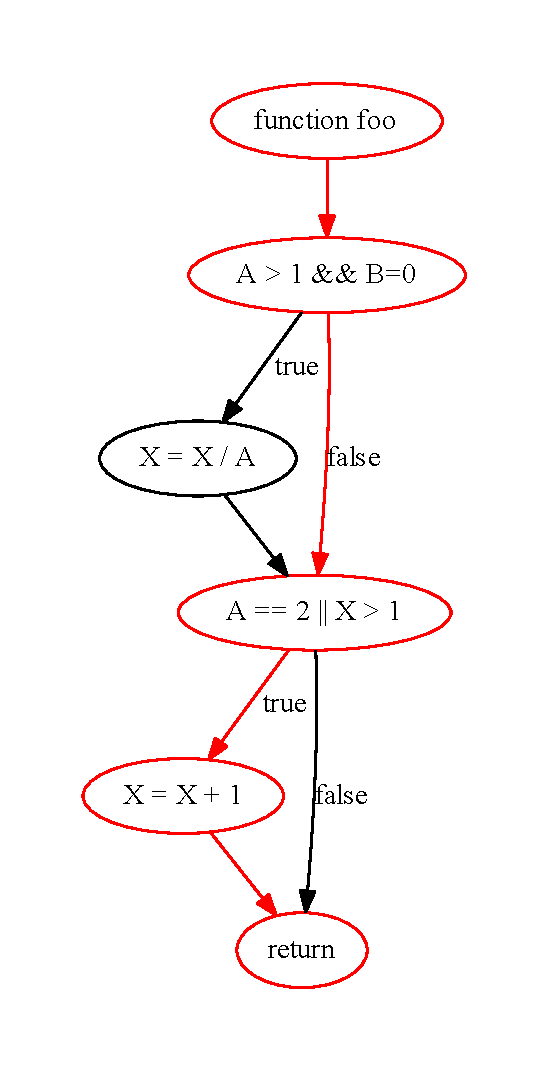
\includegraphics[scale=0.25]{figures/cfg_path1.pdf} }}%
    \qquad
    \subfloat[Path 2]{{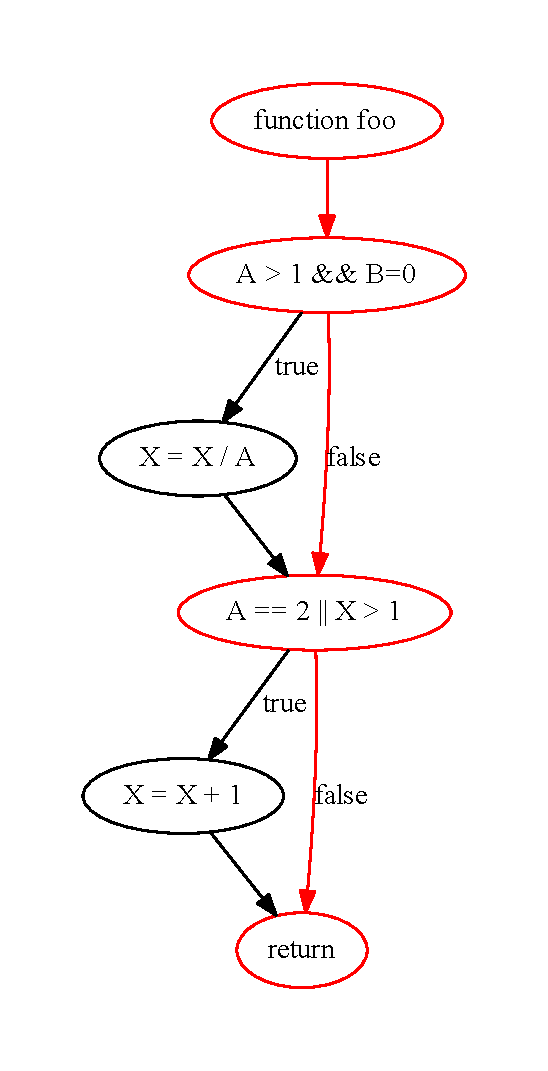
\includegraphics[scale=0.25]{figures/cfg_path2.pdf} }}%
    \qquad
    \subfloat[Path 3]{{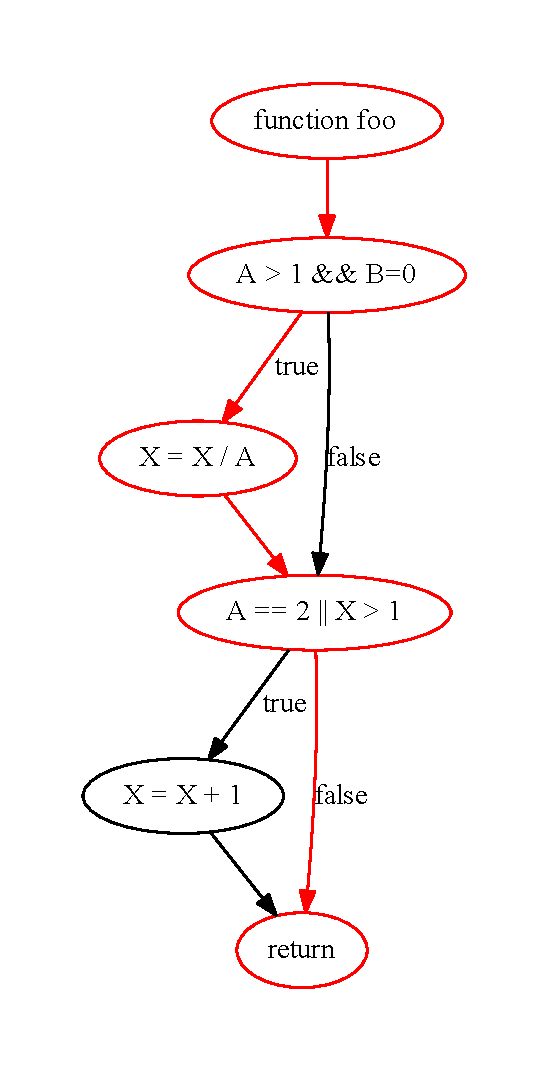
\includegraphics[scale=0.25]{figures/cfg_path3.pdf} }}%
    \qquad
    \subfloat[Path 4]{{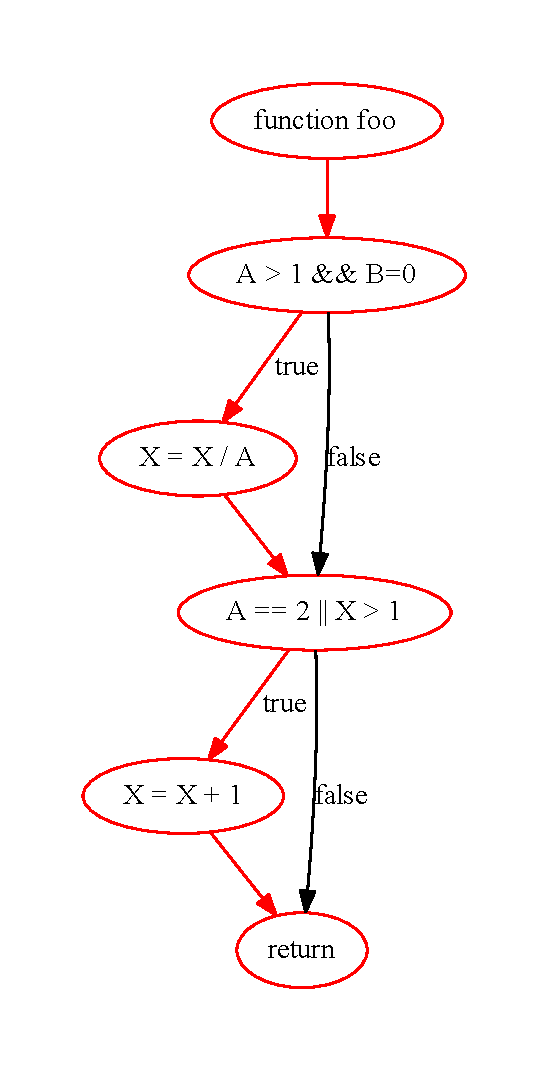
\includegraphics[scale=0.25]{figures/cfg_path4.pdf} }}%
    \caption{The possible paths through the program}%
    \label{programPaths}%
\end{figure}

Path coverage is a stronger test quality metric. Branch coverage covers all possible decisions at a program branch, but path coverage considers every possible path through the program \citep{Myers:2004:AST:983238}\citep{softwareTestingIntro}. Using the example again given by \citet{Myers:2004:AST:983238} in Figure \ref{codeCoverage}, there are four possible paths through the code. Each \verb+if+ statement can evaluate to true or false. Every path through the program therefore is when the \verb+if+ statements evaluate as follows: \verb+false, true+, \verb+false, false+, \verb+true, false+ and \verb+true, true+. Figure \ref{programPaths} colours in red the possible paths through the program.

Because \verb+if+ statements only have two possible outcomes - true or false - the number of paths through a program that only contains $n$ \verb+if+ decisions is $2^n$. However, the complexity is increased with statements such as \verb+switch+ that can have any number of paths. This is known as the cyclomatic complexity of the program, and the calculation to calculate this complexity from a control flow graph was given by \citet{1702388}:

$M = E - N + 2P$

Where M is the cyclomatic complexity, E is the number of edges in the graph, N is the number of nodes in the graph and P is the number of exit nodes. With this formula we can verify that the number of paths through the code in Figure \ref{codeCoverage} is 4. There are 7 edges, 5 nodes, and one exit point (the return statement).

$M = 7 - 5 + (2*1)$

\citet{Myers:2004:AST:983238} are even more critical of path coverage than the previous test quality metrics described. Their main points of criticism are:

\begin{enumerate}
\item The time that it would take to even generate all possible paths through a program grows exponentially with the number of branches in the program.
\item As some decisions are dependent on the outcome of previous decisions, once all possible paths have been generated it is then necessary to do further computation to calculate the actual number of possible paths through the code.
\item Even with each possible path through the code covered, there is no guarantee that the inputs used by the tests will find every problem with the code.
\end{enumerate}

In her early work on the effectiveness of path analysis, \citet{1658851} found that while the data used by tests will cause path coverage to be completed, it may not actually find bugs that are present.  therefore recommends that tests that have good path coverage are used in conjunction with boundary input data tests.

\subsection{Mutation Testing}

Mutation testing is another approach to determining the quality of a test set. Consider the following statement:

\begin{lstlisting}
y := 3x + 4 - z;
\end{lstlisting}

This is the fragment of code that we want to check that our test sets sufficiently cover. The code is called the \emph{ground string}. From the ground string, mutant strings are created. These mutant strings are based on the ground string, but have been `mutated' in some way such that they are not the same as the ground string, but still compile \citep{softwareTestingIntro}. Some example mutants might be:

\begin{lstlisting}
y := 3x - 4 - z;
y := 3x - 4 + z;
y := 10x + 6 - i;
\end{lstlisting}

The mutants all compile, but alter the outcome of executing the function. So the quality of a test set can be determined by running the set on each of the mutants and checking how many of the mutants are rejected. The perfect test set would reject all of the mutants \citep{softwareTestingIntro}. The example above is greatly simplified, and in reality it is unlikely that all of the mutants would be caught by the test set.

According to \citet{softwareTestingIntro}, in addition to being used to determine the quality of test sets, mutation testing (and path coverage and code coverage) can be used to help develop a high quality test set. He claims that there are 11 mutation operations that should be used, regardless of the programming language in question:

\begin{description}
\item[ABS] Absolute Value Insertion - Forces the tester to have at least one positive, one 0 and one negative value for the variable that has the \verb+abs+ function applied to it.
\item[AOR] Arithmetic Operator Replacement - Swapping between addition, subtraction, multiplication, division and modulus operators.
\item[ROR] Relational Operator Replacement - $<, \leq, ==, \geq, >, \neq$ operators are interchanged.
\item[COR] Conditional Operator Replacement - AND, OR, true and false are interchanged.
%\item [SOR] Shift Operator Replacement - The shift operators $\ll,\gg $and $\ggg$ are interchanged.
\item[LOR] Logical Operator Replacement - Bitwise operators AND (\&), OR ($\mid$) and exclusive OR (\^{}).
%\item[ASR] Assignment Operator Replacement - The operators $+=, -=, *=, /=, \%=, \&=, |=, \^{}=, \ll=, \gg=, \ggg=$ are replaced with one of the other operators.
\item[UOI] Unary Operator Insertion - One of the unary operators $+, -, !, ~ $ is inserted in a valid position.
\item[UOD] Unary Operator Deletion - One of the unary operators $+, -, !, ~ $ is deleted from a position where a deletion will leave the statement valid.
\item[SVR] Scalar Variable Replacement - Each reference to a variable is replaced by another variable in scope of an appropriate type.
\item[BSR] Bomb Statement Replacement - Each statement is replaced by a bomb statement that causes the program to fail.
\end{description}

\citet{softwareTestingIntro} 
\subsection{Coverage Analysis Software}

\subsection{Model Transformation Testing}

EuGENia is a model transformation written in ETL. It takes an Ecore metamodel as an input and generates gmf models as an output\citep{eugeniaSite}. One approach to verifying and possibly improving the consistency between EuGENia and EuGENia Live is to ensure that both applications have a good quality test suite.

\citet{mttBarriers} describe the three stages to model transformation testing:

\begin{enumerate}
	\item Generate test data: As with any type of test, there needs to be some input to the system. In this case it will be a set of models that are to be transformed. These models will conform to the metamodel that specifies input to the model transformation, and will either be manually created by the tester, or automatically generated in the form of graphs of metamodel instances \citep{mttBarriers}.
	\item Define test adequacy criteria: For any modeling language beyond the very basic there will be a very large number of possible inputs. This rules out running every possible model through the transformer in to test it as it would take too long. Instead a test adequacy criteria must be defined that allows the effective seletion of test models. According to \citet{mttBarriers}, there is no well-defined criteria for model transformation testing.
	\item Construct an oracle: The oracle gets the output of the system and determines if it is correct (based on the test input model).
\end{enumerate}

\citet{fleureyMTInputs} propose a general framework for assessing the quality of model transformations. Their paper begins by discussing the possibility of finding `partitions' of the transformation's input meta-model. A partition is where the model could be one of a range of values, so for example if the metamodel specifies a boolean, there is a partition as the boolean could be either true or false. With these partitions, we could check that the input test set covers each possible combination of partitions. \citet{fleureyMTInputs} then go on to state why this isn't necessarily the most useful approach: first the complexity rises quickly with each additional partition. Secondly some of combinations of partitions will not be relevant for testing, and the tester would have to find these and remove them. Finally, some relevant combinations could be missing. Generating every single combination of partition will `not ensure the existence of more than one composite state' they state.

What \citet{fleureyMTInputs} propose is the idea of model and object fragments that `define specific combinations of ranges for properties that should be covered by test models'. Their paper suggests that one of the more important aspects of model transformation testing is ensuring that input models cover the correct criteria - that they thoroughly test the transformation, while avoiding having many very similar inputs that don't test anything that has not already been tested by another input. This is of course an important aspect to consider, but for the purposes of testing EuGENia may be slightly excessive. EuGENia is not a huge transformation, and so when I decide on my test inputs I will keep this framework in mind, although I will not follow it strictly. More important I believe is the oracle aspect of testing.

The oracle can be difficult to create for any complex model transformation. \citet{mttOracleIssue} propose six ways that an oracle could be implemented for model transformation testing:

\begin{enumerate}
	\item Compare the output to a reference model (i.e. the expected output model for the particular input). Unfortunately this requires that the tester has to create the expected models for each test. For a large test set this could be incredibly time consuming.
	\item Perform an inverse transformation on the output. This would give the original input model, if the model transformation was correct. This requires that the tester implement a reverse transformation, and also requires that the transformation is an injective function (i.e. a function that preserves distinctness). According to \citet{mttOracleIssue}, this is unfortunately unlikely.
	\item Compare the output with that from a reference model transformation. This reference model transformation can produce the reference model from the test model. 
	\item A generic contract is a list of constraints on the output of the model transformation based on the input. Once the model transformation has completed the output model is checked against the constraints defined in the generic contract.
	\item The tester could provide a list of assertions in OCL (or EVL) that can be checked on the output model. Not every detail about the output model must be provided. Doing so would be a waste of time as providing the expected output model would be quicker.
	\item Model snippets could be provided by the tester. Each snippet is associated with a cardinality and logical operator so that the expected number of occurrences of each snippet can be calculated. The oracle would check that the expected number of each snippet appears in the output. 
\end{enumerate}




% Close chapter with testing of model transformations
% Barriers to systematic model transformation testing 2010
% Qualifying input test data for model transformations
% Model transformation testing : Oracle Issue

% 

\chapter{Analysis}

\section{Introduction}
In this chapter an analysis of the problem is presented, along with a development plan.

\section{The Problem}

EuGENia has a test suite written for it. However, the test suite has never been analysed, and it is therefore not known how thoroughly tested EuGENia actually is.

In the literature review, the section titled `Quality of Software Testing' discussed various approaches to determining how thorough a test set is. Based on that research, I will begin by attempting to perform statement coverage on the EuGENia transformation when the test set is executed.

Rather than implement statement analysis for just the EuGENia test suite, I will implement it for EOL in general, and attempt to detail a general approach for statement analysis in any language. As Epsilon has many languages, my documentation may prove useful for a future developer who wishes to implement statement analysis in another Epsilon language, or even a non-Epsilon language that does not yet have a statement analysis tool implemented.

In the book by \citet{Myers:2004:AST:983238}, he states that statement analysis is the easiest form of coverage analysis, but is not particularly useful. Therefore I will next consider the possibility of branch analysis which is described as more difficult, but more useful that statement coverage. Once again this will be documented in the general sense in the hope that my approach can be applied to any procedural programming language.

Again, \citet{Myers:2004:AST:983238} is critical of branch analysis, and suggests that path coverage is a better metric of coverage. However, it is more difficult to implement than branch analysis. As with statement coverage and branch analysis, I shall attempt to document the procedure for performing the analysis in the most general sense, so that future developers can perform branch analysis on any procedural programming language.

If time permits then I will attempt to implement mutation testing. However, research suggests that this is an incredibly difficult problem that may take longer to solve than the time that I have available.

For each of the above forms of analysis I have not yet specified how exactly the coverage metric will be presented to the user. In the literature review I looked at some software packages that were plugins to Eclipse that highlighted statements and branches that were covered or not covered. If time permits then I will look into creating an Eclipse plugin. However, the main focus of my project is to actually produce various coverage metrics, and so most of my time will be focused on getting those values. If I do not have much time towards the end of the project, then I will simply output a text or HTML file of some sort that details the results of the analysis.

It is assumed that the three forms of analysis (statement, branch and path) will each be dependent on the previous. So branch analysis cannot be completed until statement analysis has been completed. While this is not strictly true, it is likely that in practice that this will be the case. As I will be new to the Epsilon source code, it makes sense to implement the easiest form of coverage first. Figure \ref{ganttChart} is a Gantt chart that details the expected progress of my project. No dates are included on the Gantt chart purposefully, as it is impossible to know at this stage how long each one will take.

\begin{figure}
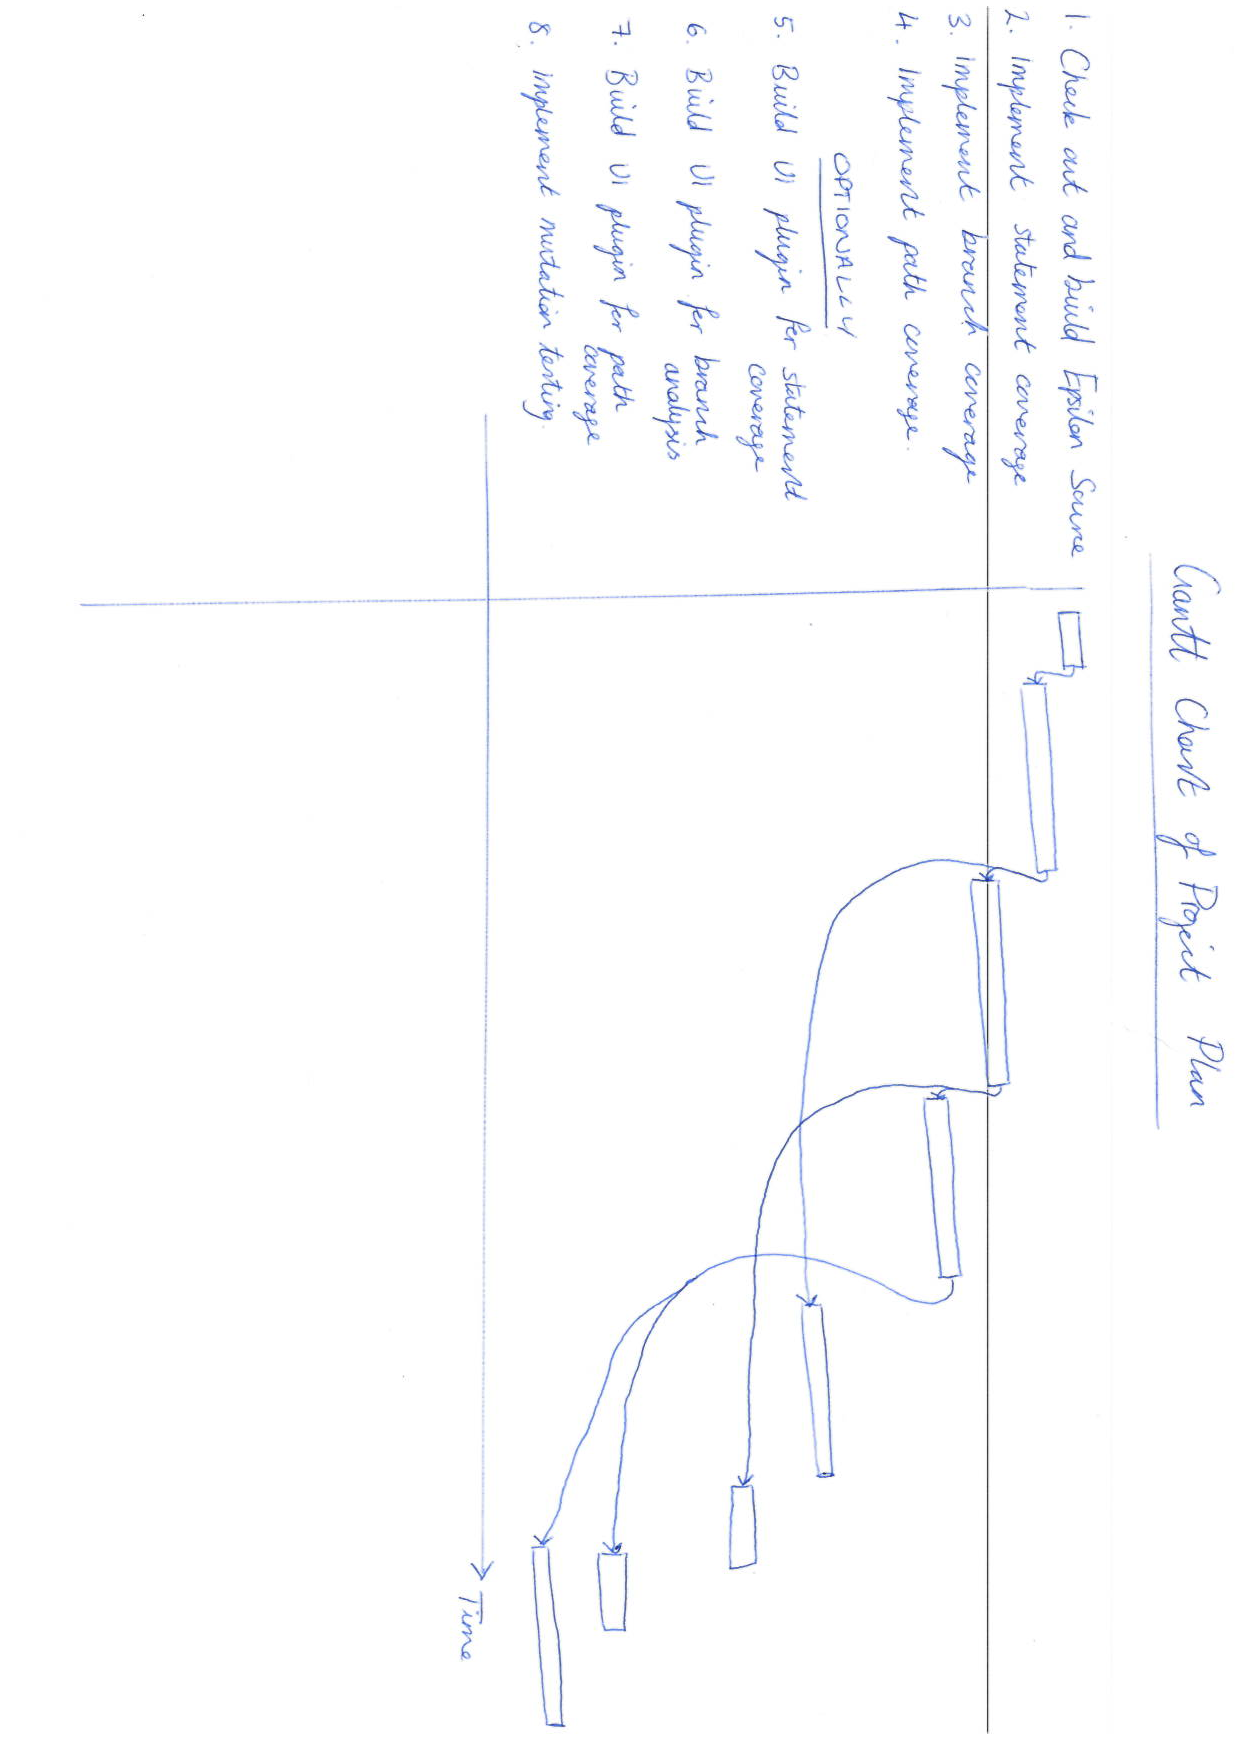
\includegraphics[scale=0.5]{figures/gantt.pdf}
\label{ganttChart}
\caption{A gantt chart of the project's expected progress}
\end{figure}
\chapter{Requirements Analysis}

\section{Introduction}

In this chapter I will perform some analysis on the requirements of this project. I will begin by identifying the stakeholders in this project, and explaining their role and general aims. From this, I will then move on to detail some derived functional requirements, followed by some derived non-functional requirements.

\section{Stakeholders}
A stakeholder in the most general sense is defined by \citet{stakeholderDef} as:

\begin{quote}
	A person, group or organization that has interest or concern in an organization
\end{quote}

More specifically in this project a stakeholder is someone or some group of people who have an interest in, or may benefit from, the contributions that my project makes to the field of model driven engineering or software testing.

I have identified the following stakeholders then from the above definition:

\begin{enumerate}
\item Enterprise Systems Group at The University of York
\item Developers who use EOL
\item Project Supervisor
\item Student
\end{enumerate}

The Enterprise Systems Group is a group of academics and research students at The University of York. As outlined on their website \cite{ESG}, the group's primary objectives are to research and teach the fundamental objectives of enterprise systems. One of their main research areas is Model-Driven Development, which is how Epsilon came to be. Any contributions that my project make will be based around Epsilon, and should it be of a high enough standard then the outcome of my project may be incorporated into the Epsilon plugin.

The developers who use EOL is a potentially large group of people. As EuGENia is a transformation that is written in EOL, and EOL is not a language that is as widely used as say Java, the approach taken to testing will be thoroughly detailed so that another developer using EOL can use this document as a reference.

The users of EuGENia have an obvious interest in the outcome of my project. Should I find any bugs in EuGENia then I will either attempt to fix them, or at least alert the relevant people (such as a developer in the Enterprise Systems Group). This will improve the experience of EuGENia for users.

My project supervisor is a stakeholder in the project in a different way than the previously listed groups. He is currently and will continue to be involved in the project until the end. He sets deadlines, makes recommendations and suggests areas to research.

The student (myself) has a stake in the project. He is the primary researcher, developer and author of documentation. However his stake ends when the project is complete, as it is assumed that he will have no long-term benefit from the outcome of the project. For this reason, no requirements should be derived from the view of the student.

\section{Functional Requirements}

\subsection{A user will be able to perform statement coverage on any EOL file}
\begin{description}[style=sameline,leftmargin=4.5cm,nolistsep]
\item[\hspace*{0.3cm}Label] F-02
\item[\hspace*{0.3cm}Description] Given an EOL file to execute, it will be possible to determine which statements within the EOL file were executed, and which were not.
\item[\hspace*{0.3cm}Source] Requirements Analysis
\item[\hspace*{0.3cm}Stakeholders] Enterprise Systems at The University of York, Developers who use EOL
\item[\hspace*{0.3cm}Satisfiable Conditions] A user can find out which statements were executed, and which were not.
\end{description}

\subsection{The output of statement analysis will tell the user what number of statements were executed}
\begin{description}[style=sameline,leftmargin=4.5cm,nolistsep]
\item[\hspace*{0.3cm}Label] F-03
\item[\hspace*{0.3cm}Description] After running the statement analysis, the output to the user will include the number of statements that were executed and the total number of statements.
\item[\hspace*{0.3cm}Source] Requirements Analysis, Literature Review
\item[\hspace*{0.3cm}Stakeholders] Enterprise Systems at The University of York, Developers who use EOL
\item[\hspace*{0.3cm}Satisfiable Conditions] The number of statements that were executed is shown, as well as the total number of statements in the input EOL file.
\end{description}

\subsection{The output of statement analysis will tell the user which statements were executed, and which were not}
\begin{description}[style=sameline,leftmargin=4.5cm,nolistsep]
\item[\hspace*{0.3cm}Label] F-04
\item[\hspace*{0.3cm}Description] After running the statement analysis, the output to the user will include which particular statements were executed, and which were not.
\item[\hspace*{0.3cm}Source] Requirements Analysis, Literature Review
\item[\hspace*{0.3cm}Stakeholders] Enterprise Systems at The University of York, Developers who use EOL
\item[\hspace*{0.3cm}Satisfiable Conditions] The statements that were executed can be distinguished from those that were not executed.
\end{description}

\subsection{A user will be able to perform branch coverage analysis on any EOL file}
\begin{description}[style=sameline,leftmargin=4.5cm,nolistsep]
\item[\hspace*{0.3cm}Label] F-05
\item[\hspace*{0.3cm}Description] Given an EOL file to execute, it will be possible to determine which branches within the EOL file were executed, and which were not.
\item[\hspace*{0.3cm}Source] Requirements Analysis
\item[\hspace*{0.3cm}Stakeholders] Enterprise Systems at The University of York, Developers who use EOL
\item[\hspace*{0.3cm}Satisfiable Conditions] A user can find out which branches were executed, and which were not.
\end{description}

\subsection{The output of branch analysis will tell the user what number of branches were executed}
\begin{description}[style=sameline,leftmargin=4.5cm,nolistsep]
\item[\hspace*{0.3cm}Label] F-06
\item[\hspace*{0.3cm}Description] After running the statement analysis, the output to the user will include the number of branches that were executed and the total number of branches.
\item[\hspace*{0.3cm}Source] Requirements Analysis, Literature Review
\item[\hspace*{0.3cm}Stakeholders] Enterprise Systems at The University of York, Developers who use EOL
\item[\hspace*{0.3cm}Satisfiable Conditions] The number of branches that were executed is shown, as well as the total number of branches in the input EOL file.
\end{description}

\subsection{The output of branch analysis will tell the user which branches were executed, and which were not}
\begin{description}[style=sameline,leftmargin=4.5cm,nolistsep]
\item[\hspace*{0.3cm}Label] F-07
\item[\hspace*{0.3cm}Description] After running the branch analysis, the output to the user will include which particular branches were executed, and which were not.
\item[\hspace*{0.3cm}Source] Requirements Analysis, Literature Review
\item[\hspace*{0.3cm}Stakeholders] Enterprise Systems at The University of York, Developers who use EOL
\item[\hspace*{0.3cm}Satisfiable Conditions] The branches that were executed can be distinguished from those that were not executed.
\end{description}

\subsection{A user will be able to perform path coverage on any EOL file}
\begin{description}[style=sameline,leftmargin=4.5cm,nolistsep]
\item[\hspace*{0.3cm}Label] F-08
\item[\hspace*{0.3cm}Description] Given an EOL file to execute, it will be possible to determine which paths within the EOL file were executed, and which were not.
\item[\hspace*{0.3cm}Source] Requirements Analysis
\item[\hspace*{0.3cm}Stakeholders] Enterprise Systems at The University of York, Developers who use EOL
\item[\hspace*{0.3cm}Satisfiable Conditions] A user can find out which paths were executed, and which were not.
\end{description}

\subsection{The output of path analysis will tell the user what number of paths were executed}
\begin{description}[style=sameline,leftmargin=4.5cm,nolistsep]
\item[\hspace*{0.3cm}Label] F-09
\item[\hspace*{0.3cm}Description] After running the path analysis, the output to the user will include the number of statements that were executed and the total number of statements.
\item[\hspace*{0.3cm}Source] Requirements Analysis, Literature Review
\item[\hspace*{0.3cm}Stakeholders] Enterprise Systems at The University of York, Developers who use EOL
\item[\hspace*{0.3cm}Satisfiable Conditions] The number of paths that were executed is shown, as well as the total number of paths through the input EOL file.
\end{description}

\subsection{The output of path analysis will tell the user which paths were executed, and which were not}
\begin{description}[style=sameline,leftmargin=4.5cm,nolistsep]
\item[\hspace*{0.3cm}Label] F-10
\item[\hspace*{0.3cm}Description] After running the path analysis, the output to the user will include which particular statements were executed, and which were not.
\item[\hspace*{0.3cm}Source] Requirements Analysis, Literature Review
\item[\hspace*{0.3cm}Stakeholders] Enterprise Systems at The University of York, Developers who use EOL
\item[\hspace*{0.3cm}Satisfiable Conditions] The paths that were executed can be distinguished from those that were not executed.
\end{description}

\section{Non-Functional Requirements}


\subsection{Statement coverage will not take an excessive amount of time to complete}
\begin{description}[style=sameline,leftmargin=4.5cm,nolistsep]
\item[\hspace*{0.3cm}Label] NF-01
\item[\hspace*{0.3cm}Description] Statement analysis will not take an excessive amount of time to complete once the code has finished executing.
\item[\hspace*{0.3cm}Source] Requirements Analysis
\item[\hspace*{0.3cm}Stakeholders] Enterprise Systems at The University of York, Developers who use EOL
\item[\hspace*{0.3cm}Satisfiable Conditions] Statement analysis completes within 5 seconds of the EuGENia transformation completing.
\end{description}

\subsection{Statement coverage will not slow down the execution of an EOL file excessively}
\begin{description}[style=sameline,leftmargin=4.5cm,nolistsep]
\item[\hspace*{0.3cm}Label] NF-02
\item[\hspace*{0.3cm}Description] Statement analysis may slow down the execution of EOL files, but not by an excessive amount.
\item[\hspace*{0.3cm}Source] Requirements Analysis
\item[\hspace*{0.3cm}Stakeholders] Enterprise Systems at The University of York, Developers who use EOL
\item[\hspace*{0.3cm}Satisfiable Conditions] Execution should not take more than twice as long as it does when statement coverage is being monitored.
\end{description}

\subsection{Branch coverage will not take an excessive amount of time to complete}
\begin{description}[style=sameline,leftmargin=4.5cm,nolistsep]
\item[\hspace*{0.3cm}Label] NF-03
\item[\hspace*{0.3cm}Description] Branch analysis will not take an excessive amount of time to complete once the code has finished executing.
\item[\hspace*{0.3cm}Source] Requirements Analysis
\item[\hspace*{0.3cm}Stakeholders] Enterprise Systems at The University of York, Developers who use EOL
\item[\hspace*{0.3cm}Satisfiable Conditions] Branch analysis completes within 5 seconds of the EuGENia transformation completing.
\end{description}

\subsection{Branch coverage will not slow down the execution of an EOL file excessively}
\begin{description}[style=sameline,leftmargin=4.5cm,nolistsep]
\item[\hspace*{0.3cm}Label] NF-04
\item[\hspace*{0.3cm}Description] Branch analysis may slow down the execution of EOL files, but not by an excessive amount.
\item[\hspace*{0.3cm}Source] Requirements Analysis
\item[\hspace*{0.3cm}Stakeholders] Enterprise Systems at The University of York, Developers who use EOL
\item[\hspace*{0.3cm}Satisfiable Conditions] Execution should not take more than twice as long as it does when branch coverage is being monitored.
\end{description}

\subsection{Path coverage will not take an excessive amount of time to complete}
\begin{description}[style=sameline,leftmargin=4.5cm,nolistsep]
\item[\hspace*{0.3cm}Label] NF-01
\item[\hspace*{0.3cm}Description] Path analysis will not take an excessive amount of time to complete once the code has finished executing.
\item[\hspace*{0.3cm}Source] Requirements Analysis
\item[\hspace*{0.3cm}Stakeholders] Enterprise Systems at The University of York, Developers who use EOL
\item[\hspace*{0.3cm}Satisfiable Conditions] Path analysis completes within 5 seconds of the EuGENia transformation completing.
\end{description}

\subsection{Path coverage will not slow down the execution of an EOL file excessively}
\begin{description}[style=sameline,leftmargin=4.5cm,nolistsep]
\item[\hspace*{0.3cm}Label] NF-02
\item[\hspace*{0.3cm}Description] Path analysis may slow down the execution of EOL files, but not by an excessive amount.
\item[\hspace*{0.3cm}Source] Requirements Analysis
\item[\hspace*{0.3cm}Stakeholders] Enterprise Systems at The University of York, Developers who use EOL
\item[\hspace*{0.3cm}Satisfiable Conditions] Execution should not take more than twice as long as it does when path coverage is being monitored.
\end{description}

This is of course not a final list of requirements. Each is subject to change throughout the project should it be necessary. However, a reasonable attempt will be made to keep to these requirements, and any changes will be justified fully.
\chapter{Statement Coverage}
\label{chap:statement}

\section{Introduction}

This chapter details my effort to implement statement coverage for EOL programs. I begin by analysing the Epsilon source code that I will be working with. I then move on to detailing the design and implementation of the solution. Then I move onto testing the solution, and finish off with a conclusion on the successes and failures of the solution.

\section{Analysis}

The Epsilon source is broken into many well-organised packages. The packages \\\verb+org.eclipse.epsilon.eol.*+ contain all of the code that is specific to the EOL language, and so these will be the primary focus of this analysis.

The package \verb+org.eclipse.epsilon.eol.execute+ unsurprisingly contains the code to execute an EOL program. To perform statement coverage, it is necessary to determine which statements have been executed. 

Some analysis of the execute package and its sub-packages has uncovered the interface \\\begin{flushright}

\end{flushright}\verb+IExecutionListener+, as shown in Figure \ref{lst:IExecutionListener}. An instance of a class that implements this interface can be added to a list of execution listeners. When a statement is about to execute, each object in the list of registered execution listeners has its \verb+aboutToExecute+ method called, and similarly after each statement has executed, each object in the list has its \verb+finishedExecuting+ method called.

\begin{figure}
\centering
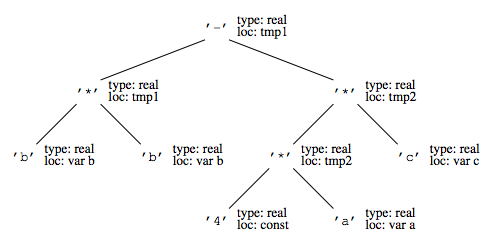
\includegraphics[width=0.5\textwidth]{figures/AST.png}
\caption{The expression b*b - 4*a*c as an AST. Taken from \citep{grune2000modern}}
\label{fig:AST}
\end{figure}
\begin{figure}
	\lstinputlisting[language=java]{code/IExecutionListener.java}
	\caption{The public interface IExecutionListener}
	\label{lst:IExecutionListener}
\end{figure}

An Abstract Syntax Tree (AST) object is provided to the execution listener. A syntax tree is the result of parsing the program text, and gives a data structure that is convenient for further processing \citep{grune2000modern}. Vertices of the AST contain a statement, and often also contain other relevant information. The EOL parser in Epsilon includes information in an AST vertex such as the type of vertex, and the line and line position of the statement that the vertex represents.

The first parameter of both methods in \verb+IExecutionListener+ is an abstract syntax tree object. The Abstract Syntax Tree class in Epsilon is designed in such a way that each vertex is an object of type AST, and each vertex has a list of children vertices, as well as a pointer back to the parent vertex. The parent vertex will have a null pointer in place of a pointer to a parent vertex, and leaf of the tree will have an empty list of children.

The AST object that is passed as a parameter into both functions is a pointer to the vertex in the program's abstract syntax tree that is about to be executed or has just been executed, depending on the method being called. 

\begin{figure}
\centering
\begin{minipage}[b]{.47\textwidth}
  \centering
  \lstinputlisting[language=EOL]{code/HelloWorld.eol}
  \caption{A simple EOL program}
  \label{lst:helloWorldEOL}
\end{minipage}%
\begin{minipage}{0.04\textwidth}
\hspace{1.00mm}
\end{minipage}
\begin{minipage}[b]{.47\textwidth}
  \centering
  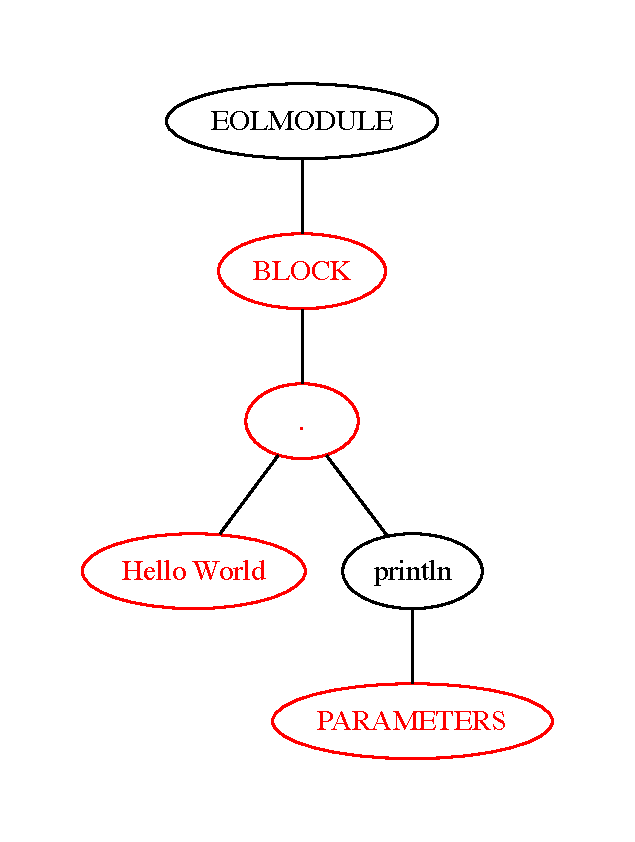
\includegraphics[scale=0.5]{figures/HelloWorldAST.pdf}
  \caption{The AST of the program in Figure \ref{lst:helloWorldEOL}}
  \label{fig:helloWorldAST}
\end{minipage}
\end{figure}

One approach for determining how many statements were executed would be to keep a list of visited AST vertices, and then count the total number of vertices in the AST. There is however a problem with this approach: Consider the very simple code in Figure \ref{lst:helloWorldEOL}, and the AST that is generated for the simple program as shown in Figure \ref{fig:helloWorldAST}. With that simple program, there is only 1 line that is going to be executed because there are no conditional statements that cause the program flow to change. However, the AST is comprised of 6 vertices. Testing shows that the execution listener's methods are only called on the red vertices. So while we know that the whole program has been executed, this naive approach will report only 4 out of 6 vertices have been executed.

Another approach that could be considered is to record which lines of the input file have been executed. This can be done because the AST class has a method called \verb+getLine()+ which as you would expect returns the line on which that statement comes from. So all of the red highlighted edges in Figure \ref{fig:helloWorldAST} return line 1 when \verb|getLine()| is called. So initial analysis would suggest that 1 out of 1 lines has been covered in the simple program in Figure \ref{lst:helloWorldEOL}, which is accurate. The problem with this was discussed in the literature review, and that is that it relies on two statements not being placed on the same line. The code in Figure \ref{lst:ifElseEOL} and its accompanying AST in Figure \ref{fig:ifElseAST} demonstrate this problem. Line coverage correctly is 100\%, because 1 out of 1 lines have been executed. However, not all of that 1 line has been executed, and so this is not an accurate reflection of the coverage. With the AST, 7 out of 14 vertices have been executed, which is a lot more accurate than the line coverage.

\begin{figure}
\centering
\begin{minipage}[b]{.44\textwidth}
  \centering
  \lstinputlisting[language=EOL,breaklines=true]{code/ifElse.eol}
  \caption{An if/else EOL program}
  \label{lst:ifElseEOL}
\end{minipage}%
\begin{minipage}[b]{.1\textwidth}
\hspace{3.00mm}
\end{minipage}
\begin{minipage}[b]{.44\textwidth}
  \centering
  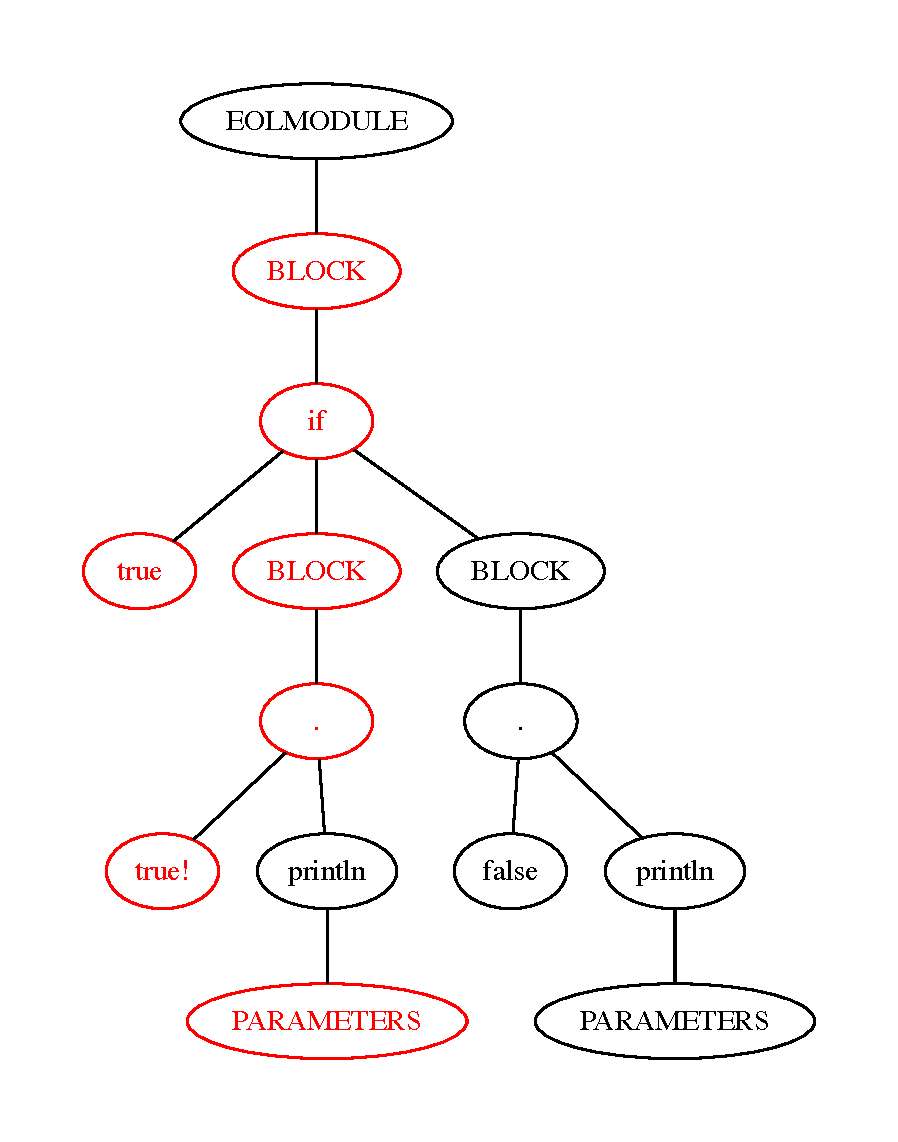
\includegraphics[scale=0.5]{figures/ifElseAST.pdf}
  \caption{The AST of the program in Figure \ref{lst:ifElseEOL}}
  \label{fig:ifElseAST}
\end{minipage}
\end{figure}

Thankfully another option is available. The AST class has a method called \verb|isImaginary()| which returns true when the current vertex is `imaginary'. While no documentation is available, it appears that vertices that can be directly mapped back to some text from the input file are not imaginary, and those that cannot be mapped back to some text are not. Figure \ref{fig:ifElseASTreal} shows the AST again, but this time with imaginary vertices left white, while non-imaginary vertices are filled in yellow. Quickly it becomes apparent that the definition of the method \verb+isImaginary()+ is not perfect as the vertex labelled EOLMODULE is coloured in yellow, despite not being directly mappable to a single statement in the input code because it instead maps to the whole program.

\begin{figure}
	\centering
	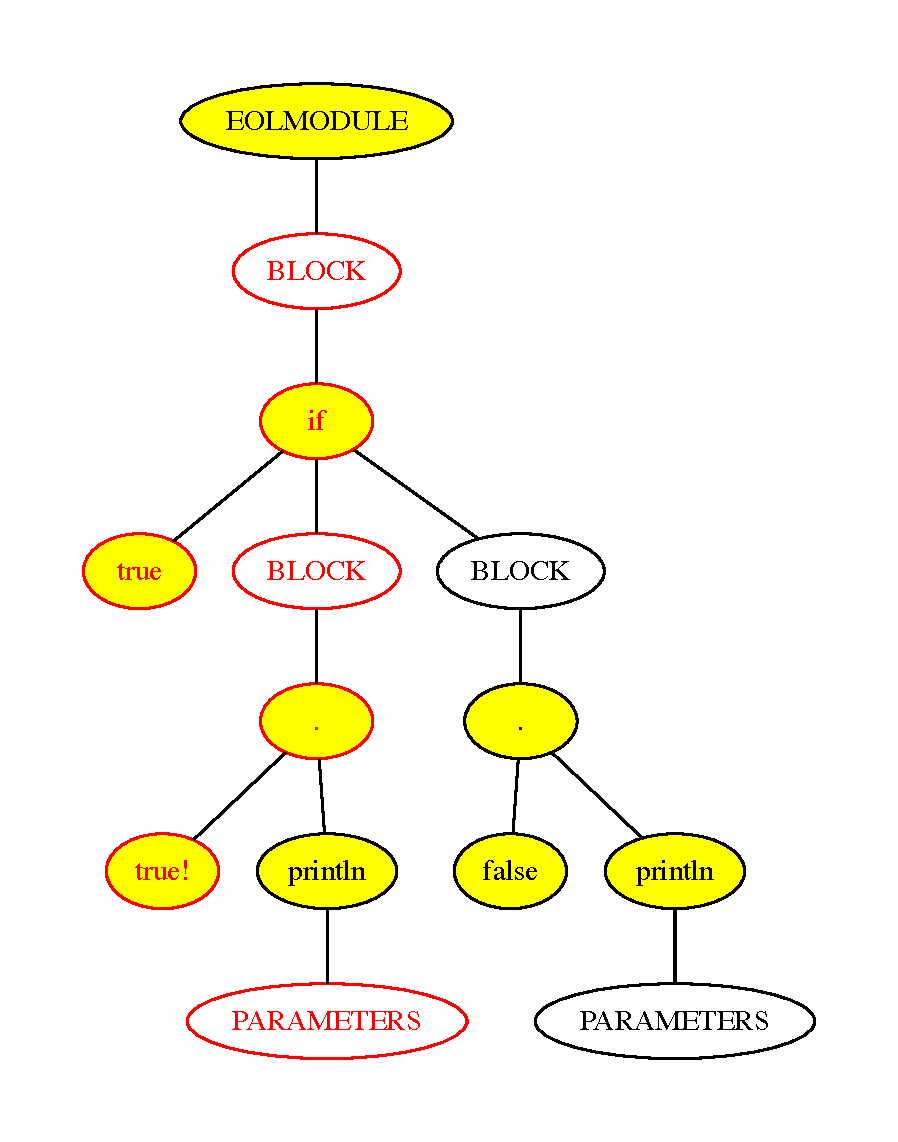
\includegraphics[scale=0.5]{figures/ifElseRealAST.pdf}
	\caption{The AST with yellow vertices being `real', and white vertices being `imaginary'}
	\label{fig:ifElseASTreal}
\end{figure}

\section{Design}

In this section I will discuss the options for the design of my solution. One of the more important aspects of the design is the performance, so that the requirements relating to performance are satisfied (NF-01, NF-02).

When the EOL executor calls the execution listener's pre or post execute methods, there needs to be a way to store a reference to the AST that is passed into either of the methods.

An obvious way of doing this would be to have a list of references to the AST. When one of the pre or post-execute methods is fired, a check would be performed on the list to see if a reference to that particular AST vertex was already stored, and if not, it would be added to the list.

Once the program has completed execution, in order to satisfy requirements F-03 and F-04, an analysis must then be performed to determine which vertices have been executed, and which have not. To do this, each vertex in the AST must be checked against the list of visited vertices. The AST can either be traversed by a depth or breadth-first algorithm. I would choose to use a depth-first algorithm purely because it is easier to implement, and uses less storage space than the breadth-first (as no queue has to be held in memory and updated).

At each recursion in the depth-first traversal, the list of visited vertices must be checked against the current vertex. This is therefore a O($n^2$) algorithm, which is not ideal as any sizeable programme can quickly slow down, which goes against requirement NF-01. 

A way around this problem would be to use a hashmap to store the visited vertices. When either the pre- or post-executed methods of the execution listener are called, a search for the AST in the hashmap would be performed to see if it has been visited or not. If not, then the AST will be inserted into the hashmap. When it comes to analysis, a depth-first search of the whole AST can be performed. At each recursive call, a search of the hashmap will be performed for that AST vertex. If it exists in the hashmap then we know that the vertex was executed.

This approach better fits the requirement NF-02, although NF-01 could potentially still not be met. If the default hashing function is poor and causes many collisions then the performance could degrade to a similar level of the previously described approach using a list of references. A solution would be to implement a better hashing function, if required.	

Both of the above solutions work around the Epsilon source code by storing information in new objects. However this is not actually a requirement - it is perfectly acceptable to modify the existing Epsilon code, as long as it is justifiable. The most simple solution then is to modify the AST class so that it contains a boolean that stores whether or not that particular vertex has been executed. When initialised of course this boolean will be set to false, but when either the pre or post-execute function in the execution listener is called and it is passed an AST as a parameter, we can just change the value of the executed boolean within the AST. This has the advantage of meaning that recording that a vertex has been visited is guaranteed to be a O(1) operation (unlike the hashmap or list based solutions). Better still, when the analysis is performed after execution has completed, the lookup time to determine whether a vertex has been executed is also guaranteed to be O(1). Again this is unlike the hashmap or linked list based solutions, which were worst case O(n) lookup time.

With the core algorithms decided on, the structure of the actual code has yet to be designed, as well as the output from the code. There of course needs to be a class that implements the \verb|IExecutionListener| interface. As the AST is directly being modified, then there is no need to transfer any data out of the execution listener (the AST will be available through another module). Therefore there needs to be a class that takes the AST as input, and produces output of some sort. So to summarise, there will be two classes implemented. One called \verb|StatementCoverageListener| that implements the execution listener interface, and another called \verb|StatementCoverageAnalyser| that analyses and outputs some information.

The format of the output must satisfy requirements F-03 and F-04, that is that it will tell the user how many statements were executed, and it will also tell the user which statements were executed, and which were not. For the latter, research detailed in the literature review of other coverage tools shows that a popular way to do this is by highlighting the statements that were executed, and either leaving statements unhighlighted that have not been executed, or highlighting them in a different colour. Most existing tools for general purpose programming languages work as plugins to an IDE such as Eclipse. However, this is a lot of work and time is limited, so initially I will find an easier approach. If time permits, then I will create the plugin after all other work is finished.

An easy way to output formatted text is to use HTML. HTML is easy to generate programmatically, and rendering the text is outsourced to a web browser. It would be possible to build my own text viewer, but it seems overly complicated when there are no disadvantages to generating a HTML page.

A class will be created that takes as input the executed AST, the file that has been executed, and the file to write the HTML to. The class will have to map executed vertices to actual characters that are in the executed file. The AST provides a function that make this relatively simple - there is a \verb|getRegion| method that allows access to the start and end positions in the file of the statement that that AST vertex maps to. From this, we need to go through the input file and mark the statements that have been executed, and those that have not. There are two possible ways to go about this. 

The first approach is to go through the executed file character by character, and go through every node in the AST and find if that particular character maps to a vertex. If it does, and that vertex has been executed, then highlighting is enabled (by changing the text background colour in HTML), and the character is copied to the output file. If the character cannot be mapped to a vertex, or it can be mapped but the vertex was not executed, then the character is simply copied across to the output file. The disadvantage of this approach is that it will be very time consuming to traverse the whole AST for every single character in the executed file. This will not help to meet requirement NF-01.

A better approach then will be to store for every character in the input text file whether or not that character should be highlighted. Initially every character will be set to not highlighted, but then the AST will be traversed, and any nodes that are not imaginary and that have been executed, the character will be set to be highlighted. Once the traversal has completed, the executed file's contents will be copied character for character. If the character being copied has been marked as highlighted, then the HTML highlighting tag will surround the character. The disadvantage of this approach is that it will require more memory than the previous approach, as it is now necessary to store more information for each character. However, it will be significantly quicker than the other approach, as the AST will only need to be traversed once.

In order to satisfy F-02, there will be a main method in the output class that takes an EOL file and output file as input, and executes the EOL file and outputs HTML to the output file.

\section{Implementation}

The first step was to modify the AST class. The additions are shown in Figure \ref{lst:ASTStatementAdditions}. Two methods (a getter and setter) have been added to modify the new boolean variable.

\begin{figure}[h]
	\lstinputlisting[language=java]{code/AST_statement.java}
	\caption{Additions to the AST class}
	\label{lst:ASTStatementAdditions}
\end{figure}

Following that, a class that implements the execution listener interface was created, and the post-execute method was completed to set the AST node to being visited.

\begin{figure}[h]
	\lstinputlisting[language=java]{code/StatementCoverageListener.java}
	\caption{The StatementCoverageClass code}
	\label{lst:StatementCoverageListener}
\end{figure}

Finally, the HTML outputter class was implemented. The whole class is too large to include here, so certain interesting parts are documented. The whole class can be found in the source that is included with this project.

% TODO add folder!

\begin{figure}[h]
	\lstinputlisting[language=java]{code/statement_HTML_core.java}
	\caption{The core of the Statement Coverage HTML output class}
	\label{lst:StatementCoverageHTMLCore}
\end{figure}

The core of the class is detailed in Figure \ref{lst:StatementCoverageHTMLCore}. Going through line-by-line, it initially reads in every line of the input file into a list of Strings. Then it next fills in the `covered array', which is an array of strings that is exactly the same in size as the list of strings that holds the input file. So for each character in the input file, there is a position in the covered array that stores whether or not the character should be highlighted. Initially all positions in the covered array are set to a 'N' character. The function \verb|dfAST| then performs a depth-first traversal of the AST of the executed program. It counts the number of non-imaginary vertices, as well as counts the number of non-imaginary executed vertices. As well it also changes the appropriate characters in the covered array to a 'Y' when an executed statement is found. 

At this stage the AST has been traversed, and it is known which characters are to be highlighted and which are not to be. Now the HTML file is written. This is started by writing the HTML header, then the page title. Then the coverage statistics are written so to satisfy requirement F-03. Next, the code from the input file is copied to the output file, and the code that has been executed is highlighted. Finally, the HTML page footers are written and the file is written to disk.

\section{Testing}
Following the implementation of the solution, it must now be thoroughly tested for bugs, and of course if any bugs are found, then the fixes will be documented here.

\begin{samepage}
\begin{description}[style=sameline,leftmargin=3.5cm,nolistsep]
\item[\hspace*{0.3cm}Label] ST-01
\item[\hspace*{0.3cm}Description] A simple program that outputs `Hello, World'.
\item[\hspace*{0.3cm}Expected Output] 100\% coverage, all code highlighted.
\item[\hspace*{0.3cm}Result] Fail
\end{description}
\end{samepage}

Unfortunately the first test has failed. The output is shown in Figure \ref{fig:ST01HTML} shows this. For the test to pass, the coverage percentage should have been 100\%, but it is showing 66\%. All of the code is highlighted, which is correct. Analysis of the AST for the sample program is shown in Figure \ref{fig:ST01AST}. As before, yellow vertices are non-imaginary vertices that can be mapped to some text of the executed file, and vertices that are outlined in red are the ones that have been marked as executed. There is code in the analyser to ignore the \verb|EOLMODULE| vertex, which is why it is only counting 3 vertices. However, rather than the \verb|println| vertex being marked as executed, its child \verb|PARAMETERS| vertex has been marked as executed. This can also be seen to be the case in Figure \ref{fig:ifElseAST}, but was not spotted at the time. 

At this stage there are a few solutions available. The first is that some code can be added to check with a \verb|println| vertex whether or not its child \verb|PARAMETERS| vertex has been executed. While a quick solution, further investigation shows that other operations also suffer from the same issue. Another potential solution is to modify the code of Epsilon so that the execution listener's post-execute method is fired on the \verb|println| vertex rather than the \verb|PARAMETERS| vertex. Unlike the simple modification that was made to the AST class earlier, this is likely to be a big job, and is probably not ideal considering that easier solutions are available. I feel then that the best solution is to modify the execution listener to detect when it has been sent a \verb|PARAMETERS| vertex to actually mark the parent vertex as executed.

\begin{figure}
\centering
\begin{minipage}[b]{.44\textwidth}
  \centering
  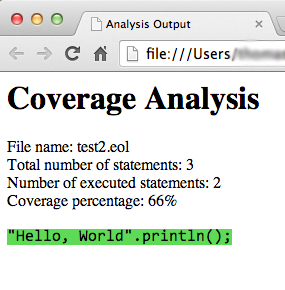
\includegraphics[width=0.6\linewidth]{figures/ST01HTML.png}
  \caption{The HTML output from test ST-01, shown in Google Chrome}
  \label{fig:ST01HTML}
\end{minipage}%
\begin{minipage}[b]{.1\textwidth}
\hspace{3.00mm}
\end{minipage}
\begin{minipage}[b]{.44\textwidth}
  \centering
  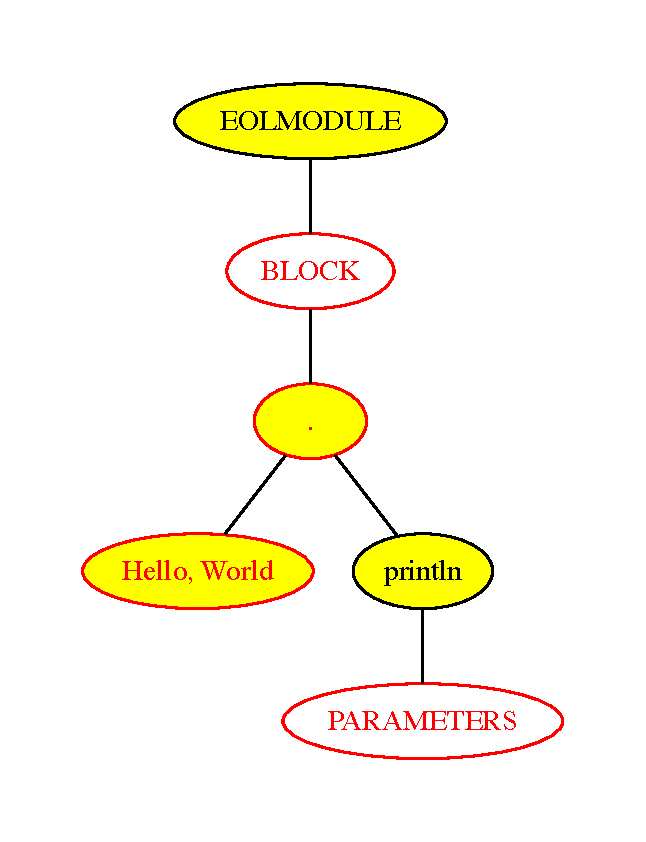
\includegraphics[width=0.6\linewidth]{figures/ST01AST.pdf}
  \caption{The AST for the program run in test ST-01}
  \label{fig:ST01AST}
\end{minipage}
\end{figure}

The code that was previously listed in Figure \ref{lst:StatementCoverageListener} has now been modified with the code shown in Figure \ref{lst:StatementCoverageST01Mod}.

\begin{figure}
	\lstinputlisting[language=java]{code/statement_ST01_mod.java}
	\caption{The updated post-execution method}
	\label{lst:StatementCoverageST01Mod}
\end{figure}

The results from re-running test ST-01 are shown in Figure \ref{fig:ST01HTMLfixed}, and the AST is shown in Figure \ref{fig:ST01ASTfixed}. The test now passes.

\begin{figure}
\centering
\begin{minipage}[b]{.44\textwidth}
  \centering
  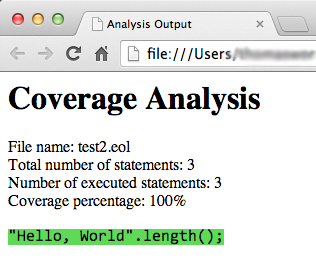
\includegraphics[width=0.6\linewidth]{figures/ST01HTML_fixed.png}
  \caption{The output after re-running test ST-01}
  \label{fig:ST01HTMLfixed}
\end{minipage}%
\begin{minipage}[b]{.1\textwidth}
\hspace{3.00mm}
\end{minipage}
\begin{minipage}[b]{.4\textwidth}
  \centering
  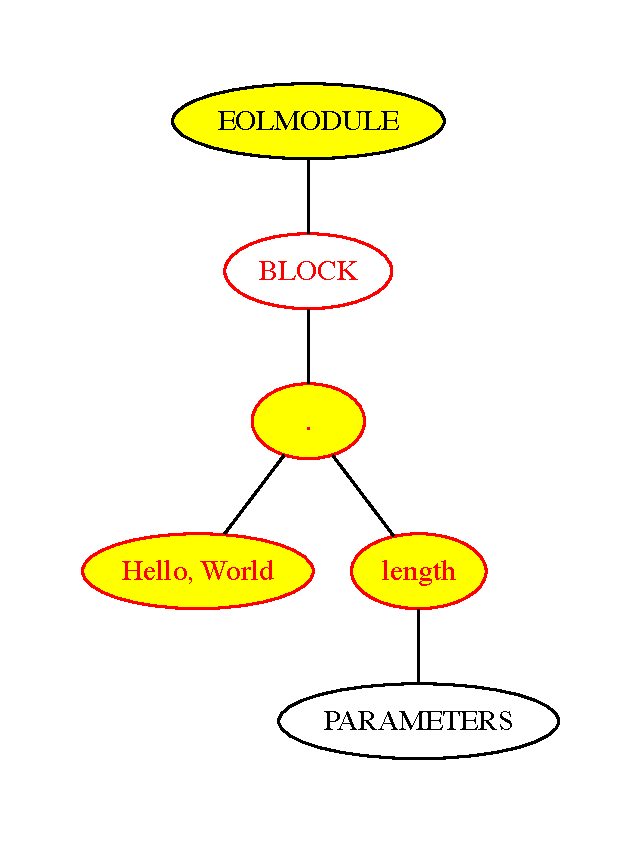
\includegraphics[width=0.6\linewidth]{figures/ST01AST_fixed.pdf}
  \caption{The AST for the program run in test ST-01}
  \label{fig:ST01ASTfixed}
\end{minipage}
\end{figure}

\begin{samepage}
\begin{description}[style=sameline,leftmargin=3.5cm,nolistsep]
\item[\hspace*{0.3cm}Label] ST-02
\item[\hspace*{0.3cm}Description] A single if-else statement, where the IF evaluates to true and so the contents of else never execute.
\item[\hspace*{0.3cm}Expected Output] Only statements within the IF block are executed, and only those statements are highlighted.
\item[\hspace*{0.3cm}Result] Pass
\end{description}
\end{samepage}

\begin{samepage}
\begin{description}[style=sameline,leftmargin=3.5cm,nolistsep]
\item[\hspace*{0.3cm}Label] ST-03
\item[\hspace*{0.3cm}Description] A single if-else statement, where the IF evaluates to false and so the contents of it never execute, but the contents of the else block do.
\item[\hspace*{0.3cm}Expected Output] Only statements within the ELSE block are executed, as well as the if evaluation.
\item[\hspace*{0.3cm}Result] Pass
\end{description}
\end{samepage}

\begin{samepage}
\begin{description}[style=sameline,leftmargin=3.5cm,nolistsep]
\item[\hspace*{0.3cm}Label] ST-04
\item[\hspace*{0.3cm}Description] A for-loop that contains a few statements, including one conditional statement that should execute on at least one iteration of the for-loop
\item[\hspace*{0.3cm}Expected Output] All statements within the for-loop should be highlighted.
\item[\hspace*{0.3cm}Result] Pass
\end{description}
\end{samepage}

\begin{samepage}
\begin{description}[style=sameline,leftmargin=3.5cm,nolistsep]
\item[\hspace*{0.3cm}Label] ST-05
\item[\hspace*{0.3cm}Description] Both a context-free and context operation are defined and called.
\item[\hspace*{0.3cm}Expected Output] All statements within each operation should be executed.
\item[\hspace*{0.3cm}Result] Pass
\end{description}
\end{samepage}

\section{Conclusions}

While the tests are highlighting the code correctly, it is notable that the covered percentage value is not actually of much use to a developer. Some statements are never actually executed, and so coverage is rarely 100\%. For ST-01 this was the case and was fixed, but further testing has shown that the problem is quite widespread. The output for ST-05 is shown in Figure \ref{fig:ST05HTML}, and the corresponding AST in \ref{fig:ST05AST}. The AST is significantly larger than in previous examples, but upon close inspection there are vertices that are classed as non-imaginary, that are not executed, despite the program being fully executed. Having considered this problem, I have concluded that the output is technically accurate, and thus meets requirement F-03. 

Furthermore, F-04 is satisfied as it is easy to distinguish which code has been executed and what has not. With test ST-05 the user will want to see that the contents of both operations have been executed, as well as the first line that calls the operations. The fact that the operation headers are not fully covered is unlikely to be of use to the developer, and so I do not believe that this is an issue.

Requirement F-02 has been satisfied, as the main method in the HTML output class takes in an EOL file and executes it. 

Anecdotal evidence suggests that NF-01 and NF-02 have also been satisfied, but formal analysis of this will be completed in the conclusion at the end of this report.

\begin{figure}
\centering
\begin{minipage}[b]{.44\textwidth}
  \centering
  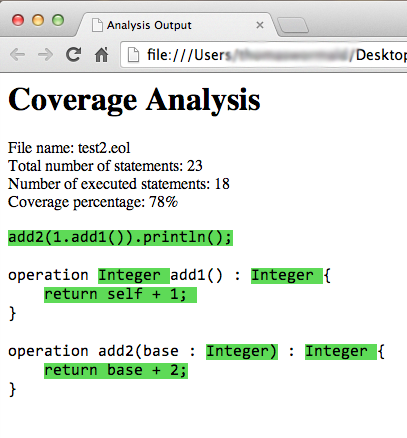
\includegraphics[width=0.6\linewidth]{figures/ST05HTML.png}
  \caption{The output after from test ST-05\\}
  \label{fig:ST05HTML}
\end{minipage}%
\begin{minipage}[b]{.1\textwidth}
\hspace{3.00mm}
\end{minipage}
\begin{minipage}[b]{.44\textwidth}
  \centering
  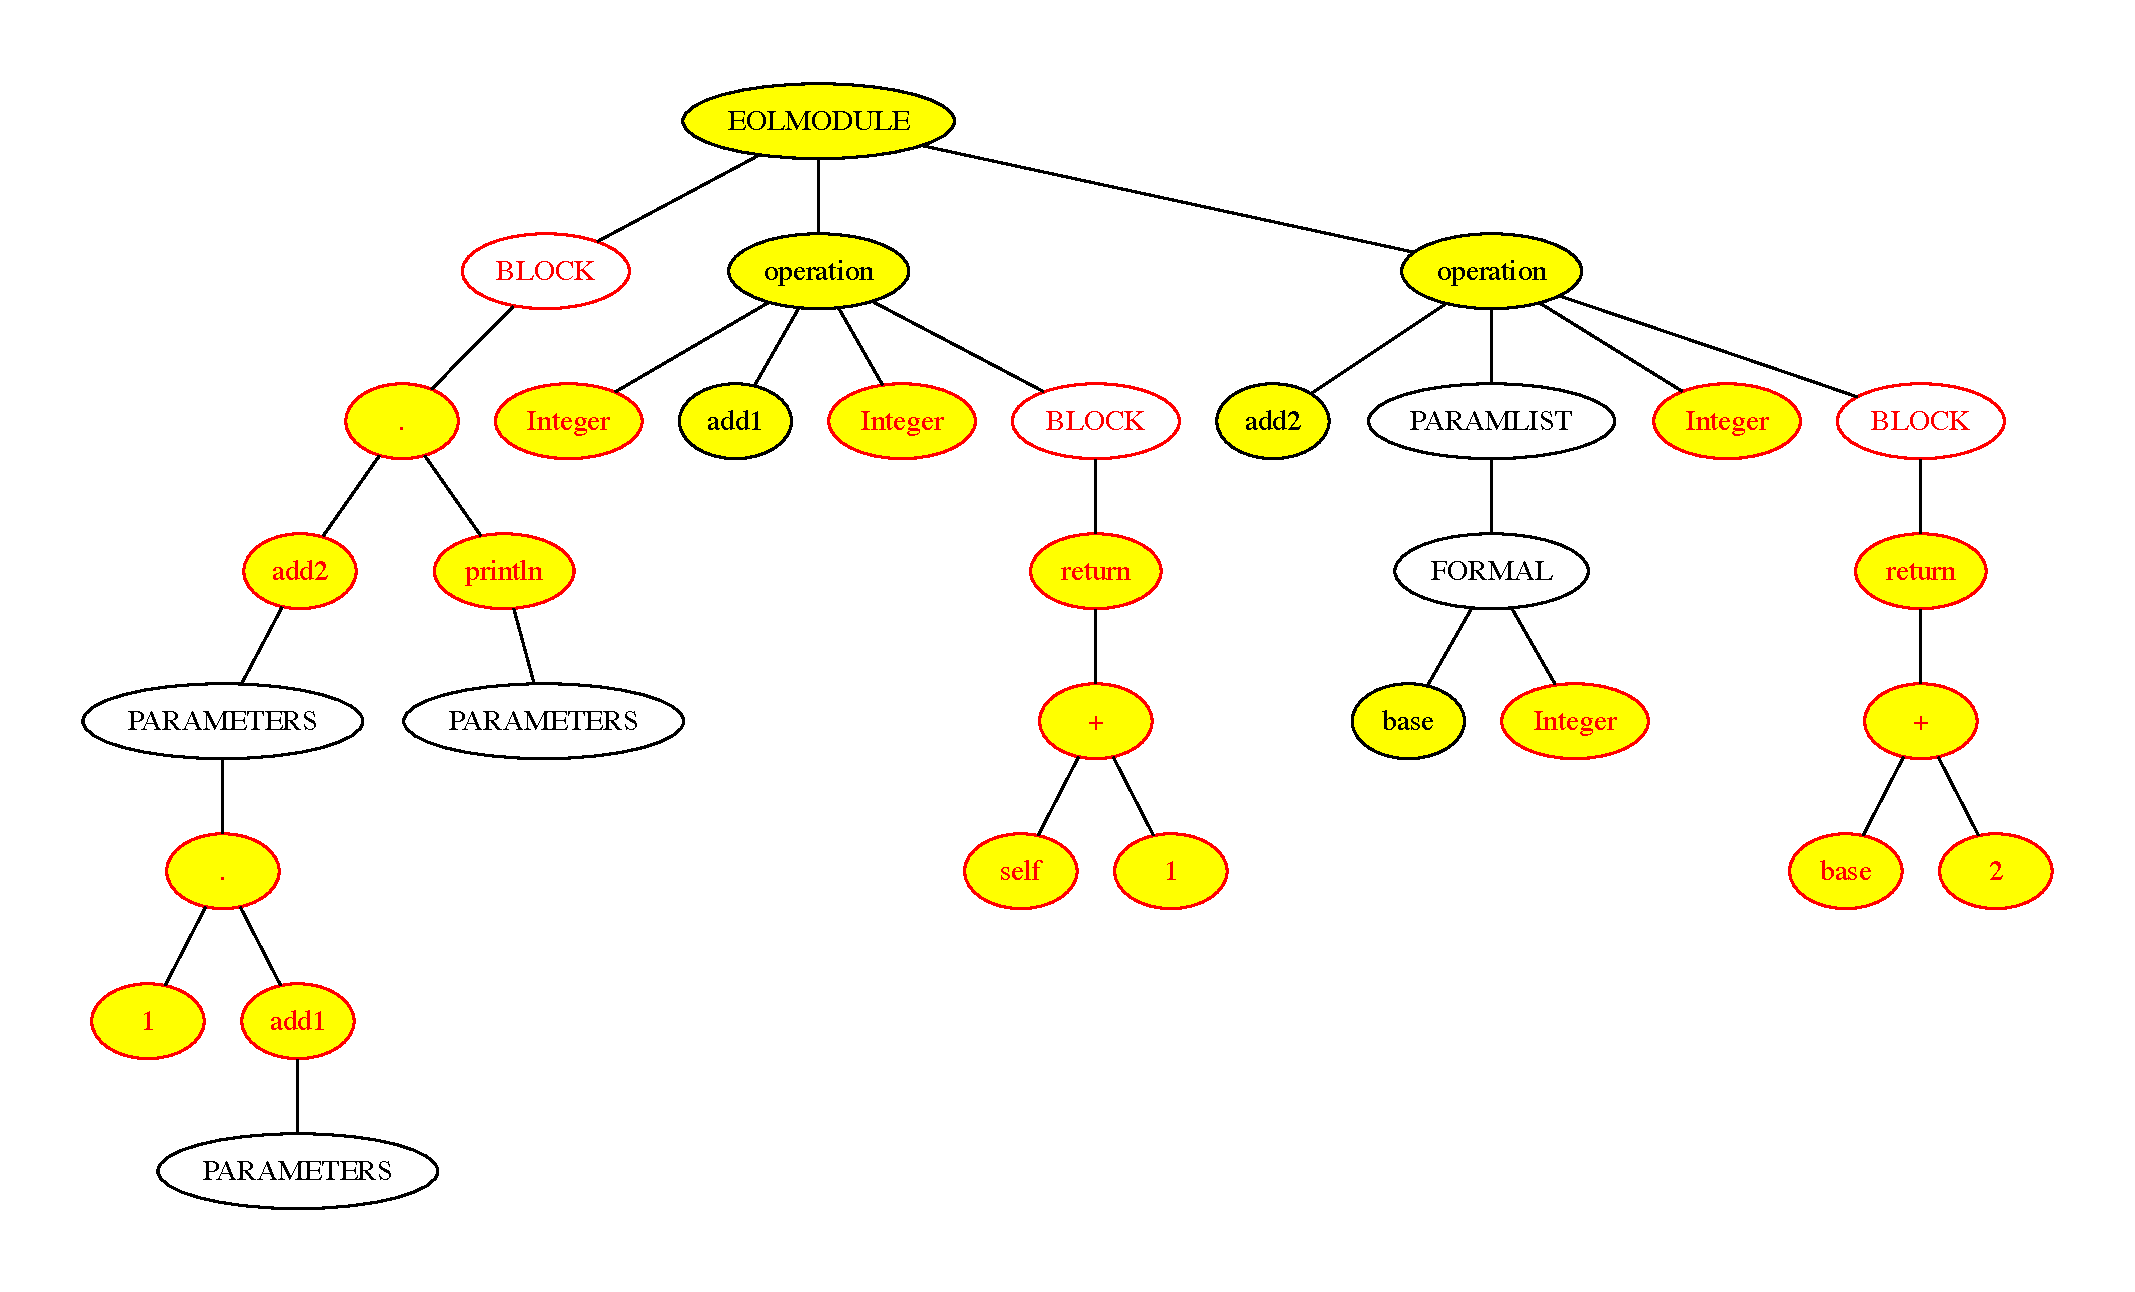
\includegraphics[width=\linewidth]{figures/ST05AST.pdf}
  \caption{The AST for the program run in test ST-05}
  \label{fig:ST05AST}
\end{minipage}
\end{figure}

On Epsilon's website \citep{epsilonWebsite} there is the JavaDoc for the source code. However, the classes that were of use to me such as AST are not documented, and so a guess had to be made about what each function did. One notable case is the \verb|isImaginary| property of an AST vertex. It seems that in most cases that vertices that can be directly mapped to a single statement in the input EOL file are not imaginary, and statement that can't (such as BLOCK) are considered imaginary. Either this assumption is incorrect, in which case some documentation is required, or there is a problem with the imaginary property because EOLMODULE is marked as not imaginary despite not being mappable to a single statement in the input file.

Another problem was found in the first test. The println function call was never passed to either of the pre- or post-execution methods in the execution listeners, but its child vertex PARAMETERS was. I suspect that this is a bug that needs fixing by the Epsilon developers. 

These problems will be added to the BugZilla website for Epsilon, so in the future this won't be a problem. I have worked around these bugs, although the workarounds are written in a way that will not cause my code to break with future updates of Epsilon that fix the bugs. 
\chapter{Branch Coverage}

\section{Introduction}
This chapter details my effort to implement branch coverage. The structure of the chapter is largely the same as the previous chapter. However, there is a lot more detail provided on the algorithm as it is thought to be the only detailed description on the process of converting an Abstract Syntax Tree into a Control Flow Graph.

\section{Analysis}

As detailed in the literature review, branch coverage is how many conditional statements have had all possible paths executed. So for an \verb|if| statement, if it only ever evaluates to \verb|true| then the branch coverage at that vertex is 50\%. This becomes a problem when you have code such as in Figure \ref{lst:branchingExample}.If the \verb|if| statement always evaluates to true during testing, statement coverage will show as being over 99\%. However, if it ever evaluates to false then \verb|someObject| won't be initialised, and an exception will be thrown later on if somewhere else \verb|someObject| is referenced.

\begin{figure}
\centering
\begin{minipage}{.4\textwidth}
  \centering
  \lstinputlisting[language=EOL]{code/branch_example.java}
  %\caption{Some sample pseudocode}
\end{minipage}%
\begin{minipage}{.5\textwidth}
  \centering
  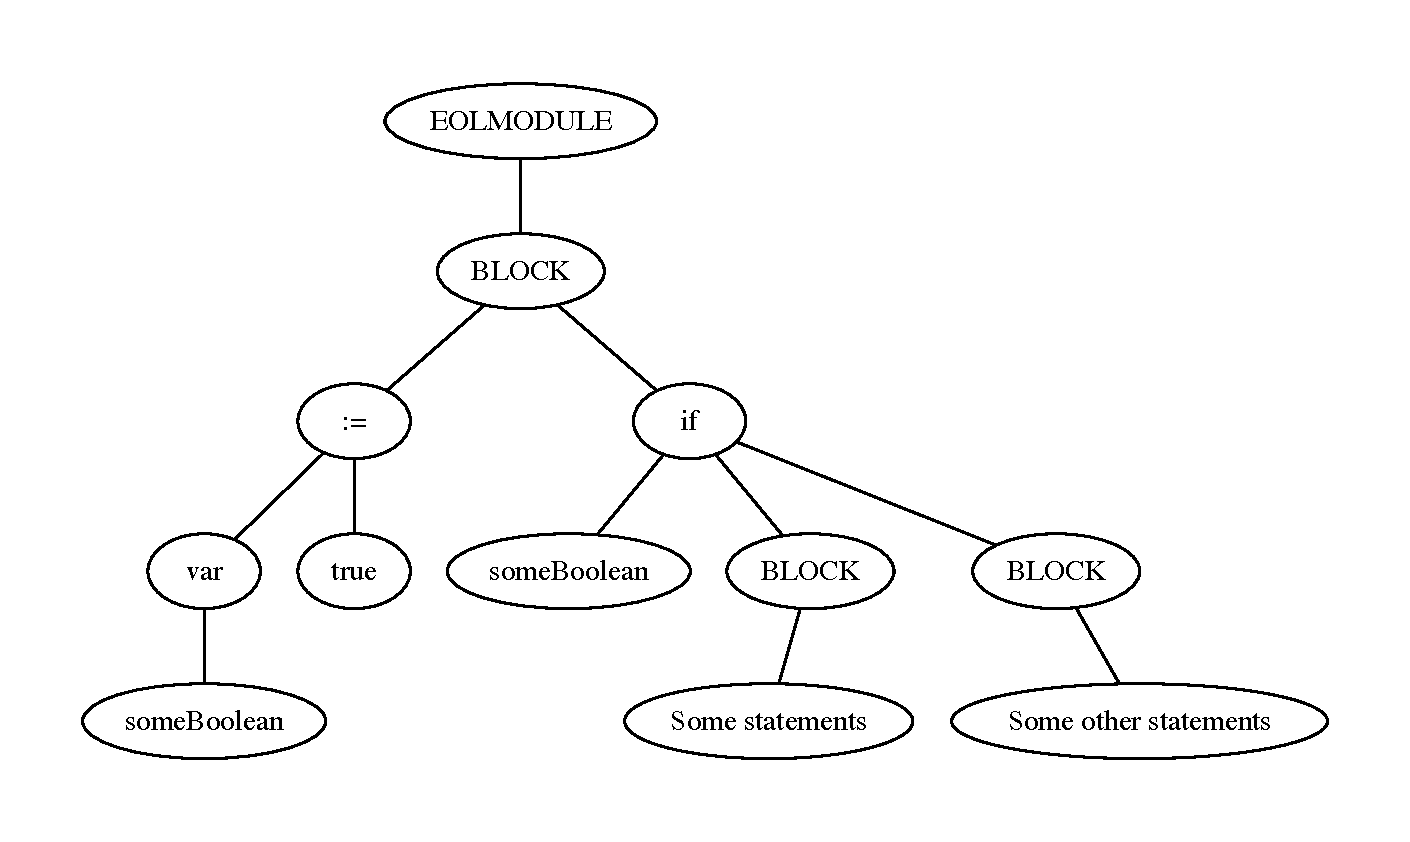
\includegraphics[scale=0.4]{figures/branchSampleAST.pdf}
  %\caption{The AST of the program in Figure \ref{lst:branchingExample}}
\end{minipage}
\caption{On the left is some sample pseudocode, and on the right is the AST for the sample pseudocode}
  \label{lst:branchingExample}
\end{figure}

Branch coverage can counter this by looking at how many of the possible paths after all conditional statements have been executed. So in the code in Figure \ref{lst:branchingExample}, only 50\% of possible paths from that \verb|if| statement have been executed, and so the branch coverage is 50\%.

By looking at the AST (Figure \ref{lst:branchingExample}) of the sample code, it would appear that by counting the number of blocks below the \verb|if| vertex, we could determine how many branches in the code there are, and after execution we could see how many of those branches have been executed.

Unfortunately this approach is not perfect. The blocks only appear when curly braces are used. If just a single statement is placed under the \verb|if| statement, then the block is skipped and just a vertex for the single statement appears. So this means that the code is now more complex than it was previously thought to be. Furthermore, \verb|if| statements can have children that never need to be executed (because they just contain information about the conditional), and so my algorithm would need to include details of this. If these were the only drawbacks then I would still choose this approach. However, this kind of caveat occurs for many conditional statements, and so the code that would be produced would be rather unwieldy and difficult to maintain.

The approach therefore that I have chosen to take is actually quite difficult to justify. I suggest that the AST be converted to a Control Flow Graph (CFG), at which point the branches from each vertex will be clear. A record will be made on which edges between vertices have been executed, and the total number of edges will be counted. The edges that have not been recorded will map to the branches that were not taken. The reason that this is difficult to justify is that an extensive search has not come up with any explicit instructions on how to go about generating a control flow graph from an abstract syntax tree. \citet{grune2000modern} very briefly discuss the process of `threading' an AST to produce a CFG, but only state that there must be a subroutine that deals with each statement. Likewise, a set of lecture slides by \citet{compilersIntro} provide some brief details on a high level algorithm, but nowhere enough to implement it from scratch.

Some forward thinking means that the conversion from AST to CFG will be necessary when performing the path coverage because of the formula detailed in the literature review's path coverage section to calculate cyclomatic complexity, and so this effort will solve two problems, and will have a quicker overall development time. Designing this algorithm and detailing it will be one of the large contributions of this project because of the lack of other detailed literature about the AST to CFG conversion process.

Before beginning development, a list was made of the statements that need to be included. This was done by going through the Epsilon book \citep{epsilonBook} which is a complete source of EOL syntax, but also as well by going through the EuGENia source (the software used in the case study in Chapter \ref{chap:evaluation}) to see which statements are actually used in real EOL code. The list was then ordered loosely in priority based on the number of uses within the EuGENia source. The list as as follows:

\begin{enumerate}[nolistsep]
\item block
\item if
\item if .. else
\item for
\item while
\item switch
	\begin{enumerate}
	\item case
	\item default
	\item continue
	\end{enumerate}
\item operation
\item return
\item break
\item breakAll
\item continue
\end{enumerate}

For each of the identified statements, I will individually analyse how they can be converted from an AST to a CFG. For each statement a sample AST will be shown, as well as the desired CFG.

\subsection{Start and End}
As discussed in the literature review, a CFG starts with a START vertex, and ends with an END vertex. In all the examples below of a CFG, these vertices are present. Each example represents a small subsection of an EOL program. When viewing the examples, the START vertex could be imagined to be where any part of a larger program joins up to the example CFG, and similarly the END vertex can be imagined to be the continue point of the program, where the statements following the example would join up to.

\subsection{The Block}
A block is not actually a statement, but refers to a block of statements. Within a block can be any other set of statements, including other blocks. The contents of a block are often contained within \{ \} braces, but not always (see the case statement).

The block is not conditional in any way. When represented in the AST, it can have any number of children, which are executed in order of first child (left-most) to last child (right-most). When a block is encountered in the AST by the conversion algorith, it should simply be a case of joining the block vertex to the last statement that was encountered, and also joining it to the block's first child.

The code in Figure \ref{fig:block} is a whole EOL program. The whole program is inside a block statement, as can be seen by the AST in the same figure. There are two statements in the block, and in the AST each statement is represented as a child. In the CFG, each of the children are represented sequentially, so the first child is represented after the block, and then the second child after the first child.

The block could be left out of the CFG, as arguably it does not provide any more information about control flow. However it is valid syntax for a block to exist as a pair of parenthesis with no statements in, and so not including the block statement could cause problems in this case. For the rest of this analysis, the block statement may be used to represent any subset of vertices that does not add to the analysis. The input to the block vertex will represent input to the first vertex of the subset, and the output from the block will represent the output from any possible exit vertices from the subset.

\begin{figure}
\centering
\begin{minipage}{.3\textwidth}
  \centering
  \lstinputlisting[language=EOL]{code/statements/block.java}
  %\caption{}
  %\label{lst:blockStatement}
\end{minipage}%
\begin{minipage}{.3\textwidth}
  \centering
  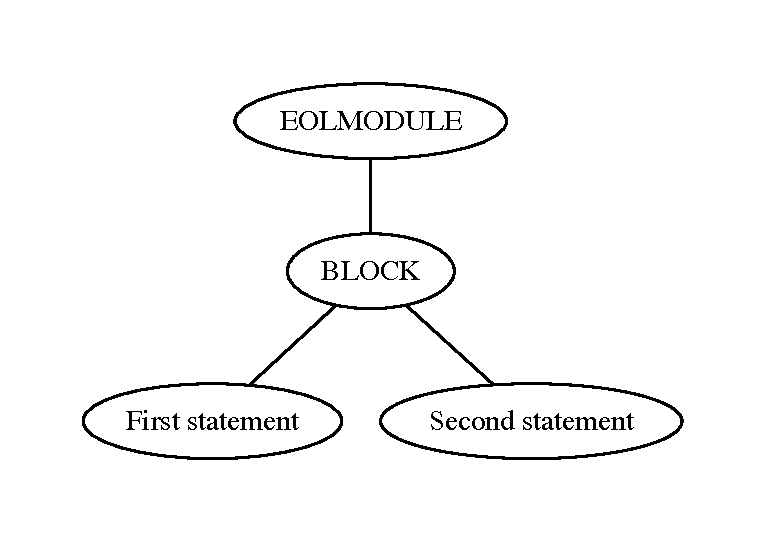
\includegraphics[width=\linewidth]{figures/statements/block_AST.pdf}
   % \caption{}
  %\label{fig:blockAST}
\end{minipage}
\begin{minipage}{.3\textwidth}
  \centering
  \includedot[scale=0.3]{figures/statements/block_CFG}
   % \caption{}
  %\label{fig:blockCFG}
\end{minipage}
\caption{From left to right: The block's code, AST and desired CFG}
\label{fig:block}
\end{figure}

\subsection{The if statement}

The if statement is going to be treated as a separate statement to the if .. else statement, because when it comes to designing and implementing the algorithm, different code will be required for each.

The \verb|if| statement evaluates its predicate, and if the predicate evaluates to true then it executes the code in the parenthesis that follow it, or if there are no parenthesis, it executes the statement that directly follows it. While the outcome of execution is the same (when there is only one statement executed following an \verb|if| statement that evaluates to true), the use of parenthesis following the if statement changes the structure of the AST in a way that must be considered during the conversion. Figure \ref{fig:if} shows the \verb|if| statement that uses parenthesis, and figure \ref{fig:ifnoparen} shows the statement that does not use parenthesis.

When the parenthesis are used, if the \verb|if| predicate evaluates to false then the statement that immediately follows the block must be the next statement to be executed. This will be the sibling of the if statement in the AST. If the if statement evaluates to true, then once it has finished executing the block it must move on to the next statement after the block, which again will be the next sibling of the if statement in the AST. This of course is assuming that a statement within either of the blocks does not divert program flow away from the next statement. A simple example would be to imagine that the contents of the block shown in Figure \ref{fig:if} are modified to include a \verb|return| statement. This is not uncommon in a program, and so must be considered. In this case the the final statement will not be executed, because return will end the current program (or sub-routine).

When no parenthesis are used, the same rules almost apply. Except that rather than looking for the next statement after the block, it will be the second statement in the statements that follow the \verb|if| statement. This will still be represented in the AST as the next sibling of the if statement.

Another consideration must be made about program flow. Within the conditional part of the if statement, any number of subroutines can exist. It could be viewed as another block of code, and this is why it appears as the first child of the if statement in the AST. For the purpose of control flow, this will be ignored. Any code within the conditional will not modify the flow of the program, as it should only evaluate to either true or false.

\begin{figure}
\centering
\begin{minipage}{.3\textwidth}
  \centering
  \lstinputlisting[language=EOL]{code/statements/if.java}
  %\caption{}
  %\label{lst:blockStatement}
\end{minipage}%
\begin{minipage}{.3\textwidth}
  \centering
  \includedot[width=\linewidth]{figures/statements/if_AST}
   % \caption{}
  %\label{fig:blockAST}
\end{minipage}
\begin{minipage}{.3\textwidth}
  \centering
  \includedot[scale=0.3]{figures/statements/if_CFG}
   % \caption{}
  %\label{fig:blockCFG}
\end{minipage}
\caption{From left to right: The if statement with parenthesis' code, AST and desired CFG}
\label{fig:if}
\end{figure}

\begin{figure}
\centering
\begin{minipage}{.3\textwidth}
  \centering
  \lstinputlisting[language=EOL]{code/statements/ifnoparen.java}
  %\caption{}
  %\label{lst:blockStatement}
\end{minipage}%
\begin{minipage}{.3\textwidth}
  \centering
  \includedot[width=\linewidth]{figures/statements/ifnoparen_AST}
   % \caption{}
  %\label{fig:blockAST}
\end{minipage}
\begin{minipage}{.3\textwidth}
  \centering
  \includedot[scale=0.3]{figures/statements/ifnoparen_CFG}
   % \caption{}
  %\label{fig:blockCFG}
\end{minipage}
\caption{From left to right: The if statement without parenthesis' code, AST and desired CFG}
\label{fig:ifnoparen}
\end{figure}

\subsection{The if .. else statement}

The if .. else statement differs from the if statement in two ways. The first is that control flow will always go down one of two paths (see Figure \ref{fig:ifelse}), rather than potentially going down one or skipping around it. Secondly, the if statement in the AST now has three children rather than just two. The additional child is the block (or single statement if no parenthesis are used) for the else statement.

When implementing the conversion a check will need to be included to see how many children the if statement has. While the EOL language parser defines an else statement, it is never featured in the AST that is generated and therefore cannot be used to distinguish between an if statement and an if .. else statement. 

Because control flow is forced down one of two paths, the final statement of both paths will now need to link to the next statement that follows the whole if .. else statement. As with the if statement, this makes the assumption that neither of the if or else blocks divert control flow. If they do, then the CFG will need to show this accordingly.

\begin{figure}
\centering
\begin{minipage}{.3\textwidth}
  \centering
  \lstinputlisting[language=EOL]{code/statements/ifelse.java}
  %\caption{}
  %\label{lst:blockStatement}
\end{minipage}%
\begin{minipage}{.3\textwidth}
  \centering
  \includedot[width=\linewidth]{figures/statements/ifelse_AST}
   % \caption{}
  %\label{fig:blockAST}
\end{minipage}
\begin{minipage}{.3\textwidth}
  \centering
  \includedot[scale=0.3]{figures/statements/ifelse_CFG}
   % \caption{}
  %\label{fig:blockCFG}
\end{minipage}
\caption{From left to right: The if .. else statement without parenthesis' code, AST and desired CFG}
\label{fig:ifelse}
\end{figure}

\subsection{The for loop}

\begin{figure}
\centering
\begin{minipage}{.3\textwidth}
  \centering
  \lstinputlisting[breaklines=true,language=EOL]{code/statements/for.java}
  %\caption{}
  %\label{lst:blockStatement}
\end{minipage}%
\begin{minipage}{.3\textwidth}
  \centering
  \includedot[width=\linewidth]{figures/statements/for_AST}
   % \caption{}
  %\label{fig:blockAST}
\end{minipage}
\begin{minipage}{.3\textwidth}
  \centering
  \includedot[scale=0.3]{figures/statements/for_CFG}
   % \caption{}
  %\label{fig:blockCFG}
\end{minipage}
\caption{From left to right: The for loop code (taken from the Epsilon Book \cite{epsilonBook}), AST and desired CFG}
\label{fig:for}
\end{figure}

The for loop in EOL works in the same way as it does in the majority of languages. It iterates over a collection of items, executing the block of code underneath it once for each element in the collection specified.

To represent the for loop in a CFG, there will initially be a for vertex. Then from the for vertex there will be the contents of the block underneath it represented (which is the third child in the example AST in Figure \ref{fig:for}).

A decision that must be made is whether the final vertex of the for loop always returns to the initial for vertex, or whether it has one edge returning to the for loop, and another edge continuing to the next statement after the for loop. For non-final iterations of the loop, the final statement within the for block will always go back to the for loop, but on the final iteration it could continue to the next part of the program. The two options are shown in Figure \ref{fig:forOptions}. The assumption that the block can be multiple statements has to be made, but you can see the two options that are available.

After some consideration (and discussion with my supervisor) I have decided to go for the option that is shown on the left in Figure \ref{fig:forOptions}. My argument is that returning to the for loop after the final iteration more accurately reflects what happens, because the program will return to the for loop to check if there are any more iterations to perform, and if not, continue on to the next statement after the for loop.

Once again statements that alter the control flow must be considered. As with the if statement, if a \verb|return| can be called within the for loop, then this must be reflected in the CFG that is generated. There are also some additional statements that must be considered. These are: \verb|break|, \verb|breakAll| and \verb|continue|, and will be discussed later.

Also to be considered with the for loop is the possibility of multiple final statements within the for statement's block. In the example in Figure \ref{fig:for}, there is an if statement that may or may not execute. If it does execute, then the final statement is the final statement within the if block. However, if it does not execute, the final statement is the \verb|if| statement, which is why I have added an edge from the if vertex back to the \verb|for| vertex. The actual implementation of this may prove to be difficult, but this will be investigated at a later time.

Up to this point, each statement has only been considered on its own. But the example in Figure \ref{fig:for} actually has an if statement within a for loop. It would be a very easy problem to solve if nested statements weren't allowed, but unfortunately it would make programs very difficult to write. Therefore the algorithm that I implement must be able to deal with any number of different types of nested statements, at any level of nesting.

\begin{figure}
\centering
\begin{minipage}{.3\textwidth}
  \centering
  \includedot[width=\linewidth]{figures/for_cfg_1}
   % \caption{}
  %\label{fig:blockAST}
\end{minipage}
\begin{minipage}{.3\textwidth}
  \centering
  \includedot[scale=0.3]{figures/for_cfg_2}
   % \caption{}
  %\label{fig:blockCFG}
\end{minipage}
\caption{The two options for the for loop}
\label{fig:forOptions}
\end{figure}

\subsection{The while loop}

The for loop iterates over a collection of objects, but the while loop iterates as long as its conditional statements evaluate to true. This is the case in most languages, and is the case in EOL. While there are some internal differences between the for and while loops in EOL (as detailed in the Epsilon Book \citep{epsilonBook}), in terms of control flow they are identical. The AST differs slightly because a for loop has 3 children, whereas a while loop only has 2. However, for control flow the only child of interest is the last one for each loop, as this is the block of statements that are executed.

Notice that the CFG example in Figure \ref{fig:while} always returns to the while vertex before continuing the program. This is the same as was decided in the for loop.

When it comes to designing the algorithm to perform the conversion, it will make sense to consider the for and while loops as the same thing, with the minor exception of the child that contains the block of statements being in a different position for each.

\begin{figure}
\centering
\begin{minipage}{.3\textwidth}
  \centering
  \lstinputlisting[breaklines=true,language=EOL]{code/statements/while.java}
  %\caption{}
  %\label{lst:blockStatement}
\end{minipage}%
\begin{minipage}{.3\textwidth}
  \centering
  \includedot[width=\linewidth]{figures/statements/while_AST}
   % \caption{}
  %\label{fig:blockAST}
\end{minipage}
\begin{minipage}{.3\textwidth}
  \centering
  \includedot[scale=0.3]{figures/statements/while_CFG}
   % \caption{}
  %\label{fig:blockCFG}
\end{minipage}
\caption{From left to right: The while loop code (taken from the Epsilon Book \cite{epsilonBook}), AST and desired CFG}
\label{fig:while}
\end{figure}

\subsection{The switch statement}

The switch statement is probably one of the most complex statements in EOL in terms of control flow. The EOL switch statement is similar to the Pascal switch statement \citep{pascalSwitch}. The switch statement takes a value as an argument, and then the case predicates within the switch statement's block are examined. If one evaluates to true, then the block that follows that case statement is executed, and control is passed to the statement that follows the block of the switch statement.

This differs from the Java switch statement, where every single case predicate is evaluated, and if it evaluates to true then it is executed \citep{pascalSwitch}. This allows for multiple case statement blocks to be executed potentially in a single switch statement.

While this is straightforward, the main complexity of the switch statement is because of the continue statement, which is now discussed.

\begin{figure}[h]
\lstinputlisting[breaklines=true,language=EOL]{code/switch_example.java}
\caption{An example of a switch statement with fallthrough}
\label{lst:switchFallthrough}
\end{figure}

If a case statement ends with continue in EOL, then the contents of every case block that follow the current case block will be executed. So in the code listing in Figure \ref{lst:switchFallthrough}, because case 0 is executed, and case 0's block finishes with the continue statement, the actual output will be:

\begin{verbatim}
Zero
One
Two
\end{verbatim}

So unlike Java's fallthrough that just checks every other case statement, it actually executes every following case statement, regardless of the case values. This complicates control flow quite a bit, because if a continue statement is contained in any of the case statements, then edges have to be added from the end that case statement and every subsequent case statement block to the start of the following case statement block.

As well as case, switch can also have the default statement within its block. The default statement is always after all of the case statements, and is executed when none of the case statements were executed (or when a continue statement was called in one of the case statements). In terms of program flow, this will remove the edge from the switch vertex to the statement following the switch block, because the default statement forces the execution of something within the switch block. As with all of the case statements, the final statement of the default block moves on to execute the next statement after the switch block.

The switch statement requires two examples to fully demonstrate possible flow. Figure \ref{fig:switch1} shows a switch statement that does not have a default statement. That means that it is possible for none of the case statements to be executed, and so there should be an edge from the switch vertex straight to the statement that follows the switch block (which in this case happens to be the end vertex because there are no more statements following the switch block). Then notice that the continue statement on the left-most case joins to the block of the next case statement, and that a vertex has been added from the end of the second case statement to the block of the third case statement.

Figure \ref{fig:switch2} shows a switch statement that does not contain a continue statement, and so the CFG on the right appears much more straightforward. Out of the switch vertex is a link to every case statement, and because there is a default statement within the switch block, there is also an edge to the default vertex. In this example there is no edge from the switch vertex to the end vertex, and this is again because the default statement is used.

\begin{figure}
\centering
\begin{minipage}{.6\textwidth}
  \centering
  \lstinputlisting[breaklines=true,language=EOL]{code/statements/switch1.java}
    \includedot[width=\linewidth]{figures/statements/switch1_AST}
  %\caption{}
  %\label{lst:blockStatement}
\end{minipage}%
\begin{minipage}{.3\textwidth}
  \centering
  \includedot[scale=0.3]{figures/statements/switch1_CFG}
   % \caption{}
  %\label{fig:blockCFG}
\end{minipage}
\caption{Top left: The example switch code that includes a continue statement. Bottom left: The AST of the example switch code. Right: The desired CFG for this example. Notice the continue statement on the left, and that there is an edge from the switch statement straight to the end statement.}
\label{fig:switch1}
\end{figure}

\begin{figure}
\centering
\begin{minipage}{.4\textwidth}
  \centering
  \lstinputlisting[breaklines=true,language=EOL]{code/statements/switch2.java}
  %\caption{}
  %\label{lst:blockStatement}
\end{minipage}%
\begin{minipage}{.3\textwidth}
  \centering
  \includedot[width=\linewidth]{figures/statements/switch2_AST}
   % \caption{}
  %\label{fig:blockAST}
\end{minipage}
\begin{minipage}{.29\textwidth}
  \centering
  \includedot[scale=0.3]{figures/statements/switch2_CFG}
   % \caption{}
  %\label{fig:blockCFG}
\end{minipage}
\caption{From left to right: The example switch statement that includes a default case, the AST for the example, and the desired CFG. Notice in the CFG that there is no edge from the switch vertex to the end vertex because there is a default vertex.}
\label{fig:switch2}
\end{figure}

\subsection{Operations}

EOL allows users to define their own operations \citep{epsilonBook}. This is a standard feature of most languages, but EOL allows two different type of operations: contextual and context-free. Context-free operations are the closest to what is found in an object-oriented language like Java. An example adapted from The Epsilon Book \citep{epsilonBook} is shown in Figure \ref{lst:contextlessOp}. The alternative is a contextual operation that extends classes with new functions. The example shown in Figure \ref{lst:contexttypeOp} shows that the operation \verb|add1()| extends the Integer class, and can be called on any object of type Integer.

This is not too important in terms of control flow, however. Both types of operations can be treated in the same way, as their AST representations are very similar, and in either case the operation is called, which is all that is important for control flow. There are three options on how these operations could be included in a CFG:

\begin{enumerate}
\item Each time the operation is called, copy all of its CFG vertices in place of the operation call. This idea can be dismissed quickly for two reasons. The first is that any operations with more than a few vertices will make the final CFG much bigger than necessary. The second is that when considering branch and path coverage, the paths through each operation only need to be considered once. If this approach was taken then the path through each operation each time it was called would have to be considered.
\item All operations will be listed just once with start and end vertices, and when a call is made to an operation, an edge will be added from the vertex that makes the call to the start of the operation, and likewise an edge will be added from the vertex that ends the operation back to the vertex that made the operation call. The problem with this approach is that during branch and path analysis, it would be implied by the CFG that the control flow can get to an operation call, execute the operation, but then return to a different part of the program (that makes the same operation call)! This is of course not an option, and so special exceptions would need to be added to the branch and path analysis code, potentially making it difficult.
\item As above, all operations are listed just once, but operation call vertices do not have any edges to the operation that is being called. While maybe this is not quite as accurate at representing program flow as the previous option, but it will simplify the process of branch and path analysis, which is the whole point of converting the program to a control flow graph in the first place.
\end{enumerate}

Figure \ref{fig:operationOptions} gives a visual representation of the options. The final option seems to be the most sensible, so this is the one that I will use in my implementation. Each operation will be treated as a separate program almost, and so branch and path analysis will work the same on them as they do on the main program flow.

\begin{figure}
\lstinputlisting[breaklines=true,language=EOL]{code/contextlessop.java}
\caption{Context-less operation}
\label{lst:contextlessOp}
\end{figure}

\begin{figure}
\lstinputlisting[breaklines=true,language=EOL]{code/contexttypeop.java}
\caption{Context-type operation}
\label{lst:contexttypeOp}
\end{figure}

\begin{figure}
\centering
\begin{minipage}{.3\textwidth}
  \centering
  \includedot[scale=0.3]{figures/operation1_CFG}
  %\caption{}
  %\label{lst:blockStatement}
\end{minipage}%
\begin{minipage}{.3\textwidth}
  \centering
    \includedot[scale=0.3]{figures/operation2_CFG}
   % \caption{}
  %\label{fig:blockAST}
\end{minipage}
\begin{minipage}{.3\textwidth}
  \centering
  \includedot[scale=0.3]{figures/operation3_CFG}
   % \caption{}
  %\label{fig:blockCFG}
\end{minipage}
\caption{Choices of how to represent an operation in a CFG. Left: option 1, where the contents of the operation's CFG are added into the main CFG each time the operation is called, so the add1 block has been included in the main CFG. The middle CFG shows option 2, that when the operation is called, edges are added to the start and end operation vertices to the call location. Finally on the right is option 3, where operations are listed as separate CFG's. }
\label{fig:operationOptions}
\end{figure}

\subsection{break, breakAll, continue and return}

These four operations have all been grouped together, because they all change program flow in a similar manner.

break in EOL is the same as break in most languages. When break is called within a loop (for or while), control breaks out of the loop and continues at the statement that follows the loop's block.

breakAll is like break, but rather than just breaking from the current loop, it will break from any number of nested loops, and continue execution after the outermost loop's block.

return ends execution of the current operation, or the main program if it is not called within an operation.

continue when used in the context of a loop has a different meaning to continue when used in a switch statement's block. In a loop, continue ends the current iteration within the loop and returns control to the loop conditional statement. 

The Epsilon Book \citep{epsilonBook} gives a nice example that uses break, breakAll and continue all in one small program. This is shown in Figure \ref{fig:break}. Notice that in the CFG, the continue statement only has an edge back to the for loop that it is contained within (i.e. the inner for loop), ending the current loop iteration. The break statement also breaks the control out of the inner for loop, and returns control to the outer for loop. Finally, the breakAll statement breaks out of both for loops, and execution is taken to the end of the program (because there are no statements after the outer for loop). No return statement is included in the example, but if it were at any point, then its only outbound edge would be to the end vertex, because it ends the current procedure or program.

\begin{figure}
\centering
\begin{minipage}{.6\textwidth}
  \centering
  \lstinputlisting[breaklines=true,language=EOL]{code/statements/break.java}
    \includedot[width=\linewidth]{figures/statements/break_AST}
  %\caption{}
  %\label{lst:blockStatement}
\end{minipage}%
\begin{minipage}{.3\textwidth}
  \centering
  \includedot[scale=0.45]{figures/statements/break_CFG}
   % \caption{}
  %\label{fig:blockCFG}
\end{minipage}
\caption{The code, AST and CFG of a program containing a continue statement, break statement and a breakAll statement.}
\label{fig:break}
\end{figure}

These four statements greatly complicate the generation of a control flow graph because they can be included nearly anywhere, and change control flow significantly. When the break is found in the example program, control flow will need to be diverted from the current loop to the statement that follows the containing for loop. Except that in this case, that's not quite right, because the for loop that is been broken out of is actually the last statement in another for loop, and as discussed in the section about for loops, at the end of a loop control should be returned to the loop header vertex, which in this case is the first for vertex.

It would be ridiculous to design an algorithm that caters for this specific case, and all other specific cases, because there are so many possible combinations and it would be near-impossible to maintain. Instead, a more clever and maintainable algorithm will be designed that can handle any combination of statements.
\section{Design}

In this section I begin by detailing the design for the AST to CFG conversion. I will then move on to discuss the design for actually performing branch analysis with the CFG.

\subsection{Representing the CFG}

The first step is to decide on how the control flow graph should be represented. At each vertex we need to store at least:

\begin{enumerate}
\item The type statement that the vertex represents
\item A label for the vertex
\item The list of children from this vertex
\item A unique ID for the vertex
\end{enumerate}

These may not be all that a vertex needs to store, but at this stage it is all that is required. An AST is similar to a CFG, and for that each vertex is stored as an object with references to child AST objects. From experience, this works well for the AST, and so the design will be loosely copied for the CFG. Each vertex of the CFG will be an object of type CFG, and will contain a list of children.

\subsection{Visualising the CFG}

Drawing a CFG will be useful for debugging, and also as a form of output to the user. Drawing a graph that organises vertices neatly that don't overlap is a difficult problem. There are existing tools that take the specification of a graph, and calculate the layout accordingly. GraphViz is one such program \citep{GraphViz} that takes a graph specification in the DOT language \citep{DOT}. The DOT language is simple, which makes the generation of graphs programmatically easy. 

\begin{figure}
\begin{minipage}{0.44\textwidth}
\lstinputlisting[breaklines=true]{figures/sampleDot.dot}
\end{minipage}
\begin{minipage}{0.44\textwidth}
\centering
\includedot[scale=0.4]{figures/sampleDot}
\end{minipage}
\caption{Left: The specification of a graph in the DOT language. Right: The graph generated from the code on the left.}
\end{figure}

GraphViz will be used for turning the CFG stored in memory into a visual representation. To convert the CFG to a DOT file, a depth first traversal of the CFG will take place. This traversal will need to keep a list of already visited vertices because the CFG can contain loops, and without the visited list the traversal could get stuck in an infinite loop.

\subsection{The Basic Case}

It makes sense to start with the most basic EOL program and convert that into a CFG. Epsilon usefully includes a tool called AST Explorer that gives a visual representation of the AST when the class EolParserWorkbench is executed. EolParserWorkbench has a string that points to an EOL file on disk, which I have modified to point to an EOL file that I can easily modify. For a simple Hello World application, the AST explorer shown in Figure \ref{fig:ASTExplorer} is shown. The AST explorer provides a lot of information, but it is not easy to quickly visualise how the tree looks, so the AST will also be visualised using graphs rendered by GraphViz. The DOT file for the AST graphs will be generated by performing a traversal of the AST and writing each recursive call as a vertex, with an edge between the last recursive call and the current one. It will differ from the CFG traversal because it won't be a directed graph, and no visited list needs to be kept, because the AST can not contain loops.

\begin{figure}
\centering
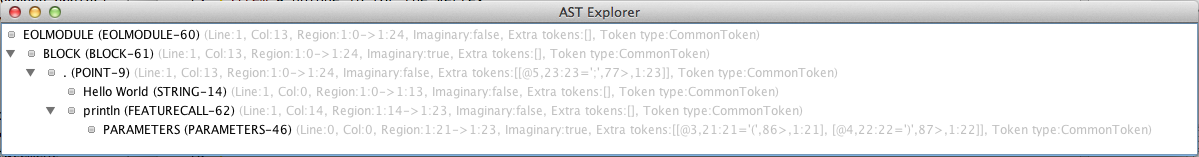
\includegraphics[width=\textwidth]{figures/ASTExplorer.png}
\caption{The AST explorer for a Hello World application}
\label{fig:ASTExplorer}
\end{figure}

The CFG for the Hello World application will have no branching points, because there are no conditional statements. The CFG for this program should look like the CFG in Figure \ref{fig:helloWorldCFG}. This looks quite similar to what happens if you perform a depth-first traversal of the AST, shown in figure \ref{fig:helloWorldDF}. Looking at the two graphs, there are differences between them. The first one is that the target CFG has a START and an END vertex. When performing the depth-first traversal, it would be simple to add a start vertex to the graph first, and link that to the root node of the AST. At each step, the last vertex found could be stored in a global variable (outside of the recursive depth-first traversal), and after the traversal has finished, the last vertex could be linked to an END vertex.

Another difference that must be addressed is that there are more vertices in the traversed AST than there are in the target CFG. This is because the AST contains all every detail of the program, so the code \verb|"Hello World".println()| is actually split into 3 vertices. The first is the string, then the point, and finally the call to the operation println. In the CFG, we are only interested in the call to the println function, the other details are not relevant to control flow. Each vertex in the AST has a type associated with it, which makes it simple to filter out types of vertices that are not relevant to the CFG. There are many different types, and so rather than blacklisting certain types, I have opted to whitelist certain types of vertices. From this hello world program, I can see that I need to add block and operation call to the whitelist.

In order to correctly join up the CFG, the use of the global variable that points to the last found AST vertex will be modified slightly. At each AST vertex, when the type is contained in the whitelist, the previously found vertex will have its child list updated to include the current vertex, and then the global pointer to the last vertex will updated to point to this vertex. This is probably easier to understand with pseudocode:

\lstinputlisting{code/ASTtoCFG_1.pseudo}

\begin{figure}
\centering
\begin{minipage}{.4\textwidth}
  \centering
    \includedot[width=0.4\linewidth]{figures/helloworld_CFG}
    \caption{The target CFG for the Hello World program}
    \label{fig:helloWorldCFG}
\end{minipage}%
\begin{minipage}{.15\textwidth}
\hspace{1cm}
\end{minipage}
\begin{minipage}{.4\textwidth}
  \centering
  \includedot[width=0.4\linewidth]{figures/helloworld2_CFG}
  \caption{The result of a depth-first traversal of the AST}
  \label{fig:helloWorldDF}
\end{minipage}
\end{figure}

At this point it hasn't been discussed how an AST object will link to a CFG object. Because the conversion code makes use of both, it needs to be easy to switch between accessing the two. One possible way of doing this is to use a hashtable with the AST vertex as a key, and a CFG object as the value. An alternative option is to modify the AST class to have an associated CFG class. Both approaches have their merits and drawbacks. The first method means that only the number of CFG objects need to be created as is absolutely necessary. However the second approach means that an AST can easily pass information into the constructor of the CFG, without it having to be dealt with by the class that is doing the conversion from AST to CFG. Because of this, I have opted to go for the latter approach, which is why in the pseudocode there is a call \verb|current.cfg| that represents getting the CFG from the AST object \verb|current|.

\subsection{The if statement}

Now that the core of the algorithm is designed, it needs to be extended to deal with statements that can send the control flow in more than one direction. I will begin by looking at the if statement, because it is one of the more simple statements.

When the depth first search reaches an if statement, it first of all needs to determine if it's an if or an if .. else statement, by looking at the number of children that it has. For the time being we assume that it has found just an if statement. The algorithm needs to add an edge from the if statement vertex to the vertex that comes after the if block. The naive approach to this would be to get the next sibling of the if statement. This doesn't work though when the if statement is the last statement within the current block. This could be fixed by looking at the parent of the sibling of the current block, but the code quickly becomes tricky to manage.

The situation is further complicated when we consider what was discussed in the analysis section about the final statement in a loop going back to the for or while loop vertex. So the problem in short then is that we don't know where the next whitelisted vertex in the AST is going to be, so we can't add an edge from the if statement to the next statement. For the time being we ignore this and look at the other path from the if statement - when it evaluates to true there will be some more vertices to add to our CFG. The depth-first traversal of the AST will add these correctly to the CFG. Because the depth-first traversal is recursive, it is quite easy to know when this process is complete. Any code that is placed after the recursive calls in a function will only be executed once the recursion has completed, so when the recursive function is called on the if statement, the CFG will have been updated after the point where the recursive call is made. In the code sample above, any code placed between the end of the foreach loop and the program end (between lines 11 and 12) would be dealing with the CFG after the if statement's children had been added to the CFG.

So why is this useful? At this point we now know that we're dealing with an if statement, and the global pointer to the last vertex to be added to the CFG points to the last vertex from the if statement's block. We still don't know where the next vertex is going to be, but we somehow need to link the if vertex and the vertex pointed to by the global last pointer to the next vertex. This can be done simply by introducing a new single vertex that mimics the next vertex and joining both vertices to it. The new vertex can be labelled `END IF' for convenience. Both paths from the if statement ultimately end up at this `END IF' vertex, and the global pointer to the last vertex is changed to point to the end if vertex. The code to do this loosely looks like this:

\begin{figure}
\centering
\begin{minipage}{.6\textwidth}
  \centering
  	\lstinputlisting{code/ASTtoCFG_2.pseudo}
    %\caption{The target CFG for the Hello World program}
    %\label{fig:helloWorldCFG}
\end{minipage}%
\begin{minipage}{.4\textwidth}
  \centering
  \includedot[width=0.75\linewidth]{figures/ifElseNoEnd}
  \caption{An incomplete if .. end CFG}
  \label{fig:ifElseNoEnd}
\end{minipage}
\end{figure}



This of course now means that there is an extra vertex in the CFG. Thankfully it can be removed once the CFG has been completed, but this will be discussed in a later section.

\subsection{The if .. else statement}

The if .. else statement complicates matters slightly. If the approach described for the if statement is applied here, then it will result in an if statement that appears to execute both the true and false blocks sequentially, regardless of the value of the if statement's parameter. To prevent this from happening, when the if .. else statement is reached by the recursive statement it can immediately add an edge from the if statement to both child blocks. The CFG class has to be then modified to add a function that blocks more parents from being added. This function will be called on the false child block of the if statement.

What then happens is the depth first search of the if statement's children occurs as usual, but when it gets to the point that the final vertex of the true block tries to add the first statement of the false block as a child, it will be prevented from doing so by the newly introduced `parent-blocking' feature. The first statement of the false block will be pointed to by the global last pointer, and the depth first traversal will continue down the if statement's children.

Once both blocks have been traversed and added to the CFG, we end up with something like what is shown in Figure \ref{fig:ifElseNoEnd}. The problem is now that we no longer have a pointer to the last vertex in the true block, because it was overwritten when the false block was traversed. A naive solution would be to add another global variable that stores the position of the last vertex within the if statement's true block. Initially it sounds like a good idea, until you think about the case where we have a nested if statement. Once the inner if statement had been traversed and added to the CFG, the end of the last vertex in the true block of the outer if statement would have been overwritten when it was used by the inner block, and so this is not a good solution.

This has been a particularly difficult problem to design a solution for, and unfortunately as a result the solution that I propose is not particularly efficient. I suggest that when an if .. else vertex is reached by the depth-first procedure, that it does a depth first traversal on each of the child blocks of the if .. else statement. After each depth-first traversal has completed, the location of the final whitelisted vertex from that child block will be stored. Once this procedure has completed, we will have the locations of the final vertices for each child block of the if statement, and these can now each have an edge added from them to an `END IF' vertex.

One final consideration must be made with the if .. else statement, which also applies to the if statement. If a break, breakAll or continue is called within either the true or false block of the if statement, then these do not want to be connected to the `END IF' statement, and so a check will have to be performed before the edge is added. 

\subsection{Loops}

As discussed in the analysis section, for and while loops will be considered as almost the same thing in the algorithm because their AST representations are very similar, and how they are to be represented in a CFG is the same.

The general case for a loop is surprisingly simple. When the recursive procedure is called with a while or for loop as its parameter, the depth-first traversal of its children can happen as normal. The contents of the loop's block are added to the loop vertex on the CFG. Once the traversal has completed, an edge is added from the global last pointer (which will point to the last vertex from the loop block) to the loop vertex. The global last pointer is then changed to point to the loop vertex, so that the next whitelisted vertex to be discovered will be added as a child to the loop vertex. This matches what was discussed in the analysis section, and the example shown in Figure \ref{fig:while}.

Once again the case where a break, breakAll or continue statement exists must be considered. They are particularly relevant in this section because each of the statements is used to change control flow within a loop. 

The break statement breaks out of the current loop. An edge must be added to the break vertex that connects it to the next statement to be executed after the while loop. To do this, when the recursive procedure is called with a break statement, it will need to find the next edge to be executed. Unfortunately with this we cannot store the location of the break vertex in a global variable and wait until the next whitelisted vertex is found because there could be multiple break statements before the next vertex is found. This could be solved by using a list, except that the next break statements to be found could be within another nested loop. Consider the following Java code.

\lstinputlisting[language=java]{code/contrivedWhile.java}

The code is rather contrived, but still valid. When the first break statement is found, it could be added to a list of discovered break statements with the intention that the the recursive function at the first statement after that while loop could check the list for any break statements, and if there were any it could remove them and add an edge from the listed break statement to the current vertex. This is fine, except that then the while loop on line 7 would be the first to check this list after the break statement on line 6 had been added. So a check could be added to see if the global last pointer points to a loop vertex. If it does, then the list is checked. However this does not work, because the increment operator statement on line 8 now satisfies that condition, and so an edge from the break on line 6 is added to the assignment on line 8! 

Unfortunately the actual solution is not a tidy one. Thinking about the position of a break statement in the AST, first of all the loop that contains the break statement must be found, which can be done by looking at the parent, then the parent's parent, the parent's parent's parent etc, until a loop is discovered. Once that happens, a check can be done to see if the loop has a sibling, and if not then the parent can be checked. If the parent is a loop then that is the statement to link the break statement to. If not, then if there is a sibling of that parent then that is the statement to link the break statement to. If not, then the checking of parents and their siblings continues until a suitable candidate is found, or until there is nothing more to check, in which case the break statement is linked to the program's end statement. This is a difficult procedure to explain, but it should become clear in the implementation section when there is some code to explain.

For the breakAll statement the process is similar, except that the outermost loop must be discovered. This is done by going through all the parents of the breakAll statement, recording the position of the last discovered for or while loop, until the root of the AST is found. Then the statement that follows the outermost loop's block is found by looking at the sibling of the loop. Again if this does not exist, then an edge is added from the breakAll statement to the end vertex of the CFG.

The continue statement is relatively simple. From the continue statement's position in the AST its parents are searched until the loop that it is contained within is found. Then an edge is added from the continue vertex in the CFG to the loop vertex. 

For each of the break, breakAll and continue statements, there can be no more children than the ones that were added once they were discovered. The depth-first traversal of the AST will continue after their discovery, but the next discovered whitelisted vertex should not be added as a child to the continue, break or breakAll vertices. The CFG class already has a `parent-blocking' feature, and now it must also have a `child-blocking' feature. This will enabled on the CFG when a break, breakAll or continue statement has been discovered and its correct child been found by the approach just described, and will prevent other children from correctly being added to those vertices.
% The child blocking feature will be sponsored by Durex
\subsection{Switch statements}

The switch statement is unique in that it can potentially any number of children from its vertex in a CFG. Remember that EOL by default is not a fallthrough switch statement, unlike Java. The first step in the conversion from AST to CFG for the switch statement is to find every case statement and add an edge from the switch vertex the discovered case vertices. As well as case statements, if a default statement is present then is should also be added as a child to the switch vertex.

Once this is done, in each case statement's block the final vertex needs to link to an `END SWITCH' block (for the same reasons as detailed in the if statement section). Unfortunately the way to do this is not particularly efficient. When each case statement is reached, a separate depth-first traversal will need to find the final whitelisted vertex within that case statement's block, and add an edge from it to the END SWITCH vertex. This could wait until the case block has been fully traversed by the normal depth-first procedure, but the end switch block would need to be kept in scope. This is more of a programming matter, and will be discussed in more detail in the implementation section.

The next consideration to make about the switch statement is that the default statement may or may not be present. If it is, then it will be included, but if it is not, then an edge must be added from the switch vertex to the END SWITCH vertex to represent the situation when none of the case statements are executed.

Finally, the continue statement within a case block has to be accounted for. If a continue statement is found, then it will have the `child-blocker' feature enabled to prevent it from linking to the END SWITCH statement. Then a the next case statement will be found by looking at the AST to find the case vertex that contains the continue statement. The next sibling of this case statement will be found, and the block vertex under the case statement will be added as a child to the continue vertex. From there, the last whitelisted statement within that case block will need to be found, and have the next case statement's block vertex added as a child. This process will repeat until there are no more case statements (or a default statement is found).

\subsection{Operations}

In the analysis section it was decided that operations will be listed as separate graphs to the main program. This means that essentially they are sub-programs, and can be treated as such when it comes to converting them from an AST to a CFG.

The AST to CFG conversion main class can be built in such a way that it takes in the root vertex of an AST, and produces a CFG from that. So when an operation definition is discovered, it's vertex can be passed into a new instance of the AST to CFG class, and the CFG that is produced can be added alongside the main program CFG when the graphical output is produced.

One small change must be made to the AST that is passed into the new instance of the AST to CFG class, and that is that the root vertex must have the link back to its actual parent removed. This is because various statements (such as breakAll) work in a way that they search as far as the root node, which is identified as the node which has no parent associated with it. If the operation vertex was passed in without removing the link back to its parent, then such searches could link to vertices that are outside of the scope of the operation definition. 


\subsection{Branch Coverage}

Once the CFG has been generated, it can be used to perform branch coverage analysis. As with statement coverage a class that implements \verb|IExecutionListener| will be implemented. A record needs to be kept about which branches have been taken. This information can be stored either in the execution listener class, or the CFG class could be modified to store it.

If the information about which branches have been executed is stored in the execution listener, then a new class will need to be defined that stores which vertex the execution started at and which one it went to. It is going to be a lot tidier to modify the CFG class to also include which branches have been executed. When the execution listener is fired on a statement, the associated CFG and parent CFG will be found, and the parent CFG will store that the child was executed.

There is a slight complication that must be considered, which is that unlike an AST, a CFG vertex can have multiple parents, but only one of them will need to store that the child has been executed. To solve this problem, a pointer to the last executed AST vertex will be stored in a global variable. The parent CFG will be accessed through the last executed AST vertex.

Once the EOL program has been executed, the number of branches in total and the number of executed branches will be counted, to satisfy requirement F-06. Satisfying F-07 is a bit more difficult, because giving a visual representation of which branches have executed is tricky. In EclEmma the branches are highlighted in Eclipse, and when you hover over them it displays how many of the branches were executed. This would be ideal, but as with statement coverage, implementing an Eclipse plugin is very time-consuming. Instead I will initially colour the edges of the output graph red if they have not been executed, or green if they have been.
\section{Implementation}

Now that an analysis and design of the conversion have been done, the implementation can be detailed. The last section of this report covered the high level algorithm details, but this section will drill down into more detail in areas where it helps for the understanding of the algorithm. All coding was done in Java because Epsilon is written in Java, and to make use of the AST class is easier if the rest of the code is in Java.

All of the code is included in the appendices. Where appropriate, small sections of code will be copied into this section, but for the most part the appendices should be referred to.

\subsection{Code Structure}

There are two main classes. The first is the class that does the conversion called \verb|AST2CFG|, and the second is the class \verb|CFG| that represents a vertex in a CFG. There is also an interface called \verb|IStatementConversion| that defines three methods. 

For each statement that must be dealt with there is a class that implements \verb|IStatementConversion|. Every class that implements \verb|IStatementConversion| has an instance added to a Hashtable, with the statement type as a key.

As earlier discussed, the core idea is a depth search algorithm, with extra code to deal with each type of statement. The main class performs a depth first search of the AST. The interface \verb|IStatementConversion| has a method defined that is called prior to the recursive depth-first search for each statement, and then another method defined that is called once the recursion has completed. 
%The conversion class can be broken down into three parts: Pre-recursion, recursion and post-recursion. To begin with, the recursive function is called with the root of the AST to be converted. Within the recursive function, a check is done to see if the node type is whitelisted. If so, it adds it as a child to the last whitelisted vertex (if there is one, if not, the start vertex is used). Then the \verb|handleAST| procedure is called with three parameters. The first is the current AST, the next is the CFG associated with the current AST (if it is whitelisted, otherwise the previously found whitelisted CFG is passed in). Finally, a list of CFG objects is passed in. Sometimes the \verb|handleAST| needs to store pointers to relevant CFG objects, and so this list is used to do that.

%Once the pre-recursion methods have finished, the recursive method is called with every child of the current AST vertex. The recursive method returns a list of CFG objects that may be of use in the post-recursive method of the parent, although it may also return an empty list. 

%Finally, the post recursive method is called. This ties up any loose ends, such as joining the end of each case statement to an END SWITCH vertex or adding the END IF statement and joining the branches of the IF statement to it.

Once the CFG has been created, a final pass is made to search for any END IF or END SWITCH statements. If any are found, then they are removed and their parent CFGs are connected to their child CFGs. If any CFGs are found that don't have a child, they are linked to the program end vertex.

\subsection{Extensibility}

%The code as it is written at the moment is not particularly extensible. Within the pre and post recursion methods a switch statement is used so that different code can be executed on different types of statement. If time permits then I will look at refactoring the code in a way that allows easy modification and maintenance. This could be useful if the conversion is changed to work on another language, such as one of Epsilon's other languages. 

The initial implementation had all of the code in the main class, and just one pre- and post-recursive method that contained the code to deal with every type of statement. Once the algorithm was implemented, this was refactored so that the code is more maintainable and extensible.

To add a new statement, it should be nearly as easy as writing a new class for that statement that implements \verb|IStatementConversion|. In this class should be the code for dealing with adding the statement to the CFG correctly. Hopefully this extensibility will make it reasonably easy to extend the conversion process to other Epsilon languages.

\subsection{Execution Listener}

The approach to recording which branches have been executed was discussed in the analysis section. There were some additional complications however that had to be catered for, and so the code is not quite as straightforward as was suggested in the analysis. One example complication is the switch statement. When a switch statement is reached, the \verb|aboutToExecute| function in the execution listener is fired for each of the case statements. This means that with the algorithm outlined in the analysis, each of the case statements is marked as executed, despite that not being true. To counter this, the code was modified to ignore case statements, and when a block was executed it was checked if it is the child of a case statement, and if so, that case statement is marked as executed.

Once execution of the EOL program has taken place, a depth first search is performed on the CFG (with a list of checked vertices to make sure that a vertex isn't visited twice, because a CFG can have loops). At each vertex, if the number of children is greater than one, then the number of children is counted, and the number of executed children is also counted. These figures are then printed to the standard output.

When the DOT file is being generated to display the CFG, if a show branch boolean is set to true, then branches are coloured in green if they have been executed, or red otherwise.

When a test is executed, most of the code will only be passed over once at most. Branch coverage is only useful if it works across multiple tests and combines the results into one graph, and so a class was created that contains stores which branches have been executed. These results can then be merged to create a CFG that contains all of the executed branches, which is used to produce the final output.
\section{Testing}

As with statement coverage, the solution must be tested. Each of the basic statements will be tested individually, and then some combinations of statements will be tested. Obviously there is an infinite number of input combinations, and only a small subsection of these can be tested. I will attempt to choose interesting inputs that require difficult to produce CFGs, rather than something less interesting, such as 10 sequential if statements. Automatic verification of the produced CFGs would be very difficult to perform, and so all CFGs will be checked by hand. This of course means that there is a risk of human error, but at this moment I can see no way to alleviate this risk.

\subsection{Individual Statements}

The criteria for a test to pass are as follows:

\begin{itemize}[nolistsep]
\item There is a START vertex at the top of the CFG which has no parents, and at least one child.
\item There is an END vertex that has at least one parent, and no children.
\item The produced CFG matches the one that was shown in the analysis section for that statement.
\item Other than the end vertex, all vertices have at least one child
\end{itemize}

\begin{figure}
\centering
\begin{minipage}{.25\textwidth}
  \centering
  \includedot[scale=0.3]{figures/branchtest/block}
  \caption{}
  \label{fig:testBlock}
\end{minipage}%
\begin{minipage}{.25\textwidth}
  \centering
  \includedot[scale=0.3]{figures/branchtest/if}
  \caption{}
  \label{fig:testIf}
\end{minipage}%
\begin{minipage}{.25\textwidth}
  \centering
    \includedot[scale=0.3]{figures/branchtest/ifElse}
    \caption{}
  	\label{fig:testIfElse}
\end{minipage}
\begin{minipage}{.24\textwidth}
  \centering
  \includedot[scale=0.3]{figures/branchtest/for}
  \caption{}
  \label{fig:testFor}
\end{minipage}
\end{figure}

Testing begins with the block vertex. This will be done by having a single line of code in a program, with no conditional statements.

\begin{samepage}
\begin{minipage}{.6\textwidth}
\begin{description}[style=sameline,leftmargin=4.5cm,nolistsep]
\item[\hspace*{0.3cm}Label] BT-01
\item[\hspace*{0.3cm}Statement under Test] BLOCK
\item[\hspace*{0.3cm}Expected Output] See figure \ref{fig:block}
\item[\hspace*{0.3cm}Result] Pass (see Figure \ref{fig:testBlock})
\end{description}
\end{minipage}
\begin{minipage}{.39\textwidth}
  \centering
  Code used for testing:
  \lstinputlisting[language=EOL]{code/branchtest/block.eol}
\end{minipage}
\end{samepage}

Of note about this test is that the operation call \verb|println| is printed, but not the string that is to be printed. This is because the type string is not on the whitelist, but the operation call type is. If both were on the whitelist, then two vertices would be used to represent that line of code.

\begin{samepage}
\begin{minipage}{.6\textwidth}
\begin{description}[style=sameline,leftmargin=4.5cm,nolistsep]
\item[\hspace*{0.3cm}Label] BT-02
\item[\hspace*{0.3cm}Statement under Test] if
\item[\hspace*{0.3cm}Expected Output] See figure \ref{fig:if}
\item[\hspace*{0.3cm}Result] Pass (see Figure \ref{fig:testIf})
\end{description}
\end{minipage}
\begin{minipage}{.39\textwidth}
  \centering
  Code used for testing:
  \lstinputlisting[language=EOL]{code/branchtest/if.eol}
\end{minipage}
\end{samepage}

The if statement does not require any code in its block for this test, because leaving the space between the parenthesis empty produces a block vertex, which is enough for this test. The if statement above will always execute because its parameter is \verb|true|, but again for testing this is not relevant because the generated CFG does not take this into account.

\begin{samepage}
\begin{minipage}{.6\textwidth}
\begin{description}[style=sameline,leftmargin=4.5cm,nolistsep]
\item[\hspace*{0.3cm}Label] BT-03
\item[\hspace*{0.3cm}Statement under Test] if .. else
\item[\hspace*{0.3cm}Expected Output] See figure \ref{fig:ifelse}
\item[\hspace*{0.3cm}Result] Pass (see Figure \ref{fig:testIfElse})
\end{description}
\end{minipage}
\begin{minipage}{.39\textwidth}
  \centering
  Code used for testing:
  \lstinputlisting[language=EOL]{code/branchtest/ifElse.eol}
\end{minipage}
\end{samepage}

\begin{samepage}
\begin{minipage}{.6\textwidth}
\begin{description}[style=sameline,leftmargin=4.5cm,nolistsep]
\item[\hspace*{0.3cm}Label] BT-04
\item[\hspace*{0.3cm}Statement under Test] for
\item[\hspace*{0.3cm}Expected Output] See figure \ref{fig:for}
\item[\hspace*{0.3cm}Result] Pass (see Figure \ref{fig:testFor})
\end{description}
\end{minipage}
\begin{minipage}{.39\textwidth}
  \centering
  Code used for testing:
  \lstinputlisting[language=EOL]{code/branchtest/for.eol}
\end{minipage}
\end{samepage}

\begin{figure}
\centering
\begin{minipage}{.25\textwidth}
  \centering
  \includedot[scale=0.3]{figures/branchtest/while}
  \caption{}
  \label{fig:testWhile}
\end{minipage}%
\begin{minipage}{.25\textwidth}
  \centering
  \includedot[scale=0.3]{figures/branchtest/switch1}
  \caption{}
  \label{fig:testSwitch1}
\end{minipage}%
\begin{minipage}{.25\textwidth}
  \centering
    \includedot[scale=0.3]{figures/branchtest/switch2}
    \caption{}
  	\label{fig:testSwitch2}
\end{minipage}
\begin{minipage}{.24\textwidth}
  \centering
  \includedot[scale=0.3]{figures/branchtest/operation}
  \caption{}
  \label{fig:testOperation}
\end{minipage}
\end{figure}

\begin{minipage}{.6\textwidth}
\begin{description}[style=sameline,leftmargin=4.5cm,nolistsep]
\item[\hspace*{0.3cm}Label] BT-05
\item[\hspace*{0.3cm}Statement under Test] switch (with fallthrough, without a default statement)
\item[\hspace*{0.3cm}Expected Output] See figure \ref{fig:switch1}
\item[\hspace*{0.3cm}Result] Pass (see Figure \ref{fig:testSwitch1})
\end{description}
\end{minipage}
\begin{minipage}{.39\textwidth}
  \centering
  Code used for testing:
  % This line breaks the document for some reason
  \lstinputlisting[language=EOL]{code/branchtest/switch1.eol}
  %\lstinputlisting{code/branchtest/switch1.eol}
\end{minipage}

\begin{minipage}{.6\textwidth}
\begin{description}[style=sameline,leftmargin=4.5cm,nolistsep]
\item[\hspace*{0.3cm}Label] BT-06
\item[\hspace*{0.3cm}Statement under Test] switch (without fallthrough, with a default statement)
\item[\hspace*{0.3cm}Expected Output] See figure \ref{fig:switch2}
\item[\hspace*{0.3cm}Result] Pass (see Figure \ref{fig:testSwitch2})
\end{description}
\end{minipage}
\begin{minipage}{.39\textwidth}
  \centering
  Code used for testing:
  \lstinputlisting[language=EOL]{code/branchtest/switch2.eol}
\end{minipage}

Both context-free and context-type operations were tested in the following test. Using the example from The Epsilon Book \citep{epsilonBook} one operation of each type was defined, and then both operations called.

\begin{minipage}{.6\textwidth}
\begin{description}[style=sameline,leftmargin=4.5cm,nolistsep]
\item[\hspace*{0.3cm}Label] BT-07
\item[\hspace*{0.3cm}Statement under Test] Operation call
\item[\hspace*{0.3cm}Expected Output] See figure \ref{fig:testOperation}
\item[\hspace*{0.3cm}Result] Pass (see right-hand CFG of Figure \ref{fig:operationOptions}). See below.
\end{description}
\end{minipage}
\begin{minipage}{.39\textwidth}
  \centering
  Code used for testing:
  \lstinputlisting[language=EOL,breaklines=true]{code/branchtest/operation.eol}
\end{minipage}

Notice that the operations are actually shown in the wrong order in the generated CFG. \verb|add1| would be executed first, because it is passed as a parameter to \verb|add2|. Looking at the AST for this code it is easy to see why. \verb|add1| is a child of \verb|add2|, because it is a parameter. When a depth-first traversal is performed, \verb|add2| is found before \verb|add1|, and so it is added to the CFG first. While this is technically incorrect, for purposes of calculating branch coverage it does not matter. However, for the more general purpose use, the operation call function would need to traverse its children to find any other operation call vertices, and add them to the CFG in reverse order. This could be done easily by recursively calling a function on the children of the AST vertex, and after the recursion checking to see if the type is an operation call. If so, then add it to the CFG and update the global last pointer to that vertex.

\begin{figure}
\centering
\begin{minipage}{.25\textwidth}
  \centering
  \includedot[scale=0.3]{figures/branchtest/break}
  \caption{}
  \label{fig:testBreak}
\end{minipage}%
\begin{minipage}{.25\textwidth}
  \centering
  \includedot[scale=0.3]{figures/branchtest/breakAll}
  \caption{}
  \label{fig:testBreakAll}
\end{minipage}%
\begin{minipage}{.25\textwidth}
  \centering
    \includedot[scale=0.3]{figures/branchtest/continue}
    \caption{}
  	\label{fig:testContinue}
\end{minipage}
\end{figure}
For the break, breakAll and continue statements, they were placed in an if statement so that the control flow was also created for when they are not executed. In separate testing that is not documented due to space constraints, they were also tested on their own and proved to work as expected.

\begin{minipage}{.6\textwidth}
\begin{description}[style=sameline,leftmargin=4.5cm,nolistsep]
\item[\hspace*{0.3cm}Label] BT-08
\item[\hspace*{0.3cm}Statement under Test] Break
\item[\hspace*{0.3cm}Expected Output] See figure \ref{fig:}
\item[\hspace*{0.3cm}Result] Pass (see right-hand CFG of Figure \ref{fig:testBreak}). See below.
\end{description}
\end{minipage}
\begin{minipage}{.39\textwidth}
  \centering
  Code used for testing:
  \lstinputlisting[language=EOL,breaklines=true]{code/branchtest/break.eol}
\end{minipage}

For break, a nested while loop was used to prove that the break statement only breaks out of one while loop, unlike the breakAll statement.

\begin{minipage}{.6\textwidth}
\begin{description}[style=sameline,leftmargin=4.5cm,nolistsep]
\item[\hspace*{0.3cm}Label] BT-09
\item[\hspace*{0.3cm}Statement under Test] BreakAll
\item[\hspace*{0.3cm}Expected Output] See figure \ref{fig:}
\item[\hspace*{0.3cm}Result] Pass (see Figure \ref{fig:testBreakAll}). See below.
\end{description}
\end{minipage}
\begin{minipage}{.39\textwidth}
  \centering
  Code used for testing:
  \lstinputlisting[language=EOL,breaklines=true]{code/branchtest/breakAll.eol}
\end{minipage}

For breakAll, a two while loops were used to prove that the breakAll statement can break out of more than just the one loop that the break statement does.

\begin{minipage}{.6\textwidth}
\begin{description}[style=sameline,leftmargin=4.5cm,nolistsep]
\item[\hspace*{0.3cm}Label] BT-10
\item[\hspace*{0.3cm}Statement under Test] Continue
\item[\hspace*{0.3cm}Expected Output] See figure \ref{fig:continue}
\item[\hspace*{0.3cm}Result] Pass (see Figure \ref{fig:testContinue}). See below.
\end{description}
\end{minipage}
\begin{minipage}{.39\textwidth}
  \centering
  Code used for testing:
  \lstinputlisting[language=EOL,breaklines=true]{code/branchtest/continue.eol}
\end{minipage}

\subsection{Multiple Statements Testing}

During the previous section I showed that individual statements are dealt with as they should be. Some of the tests also had multiple statements in, such as the break statement. Now that this has been proven, bigger test case will be executed. During development of course many were tested, but once again due to the space constraints in this document I can only record one of them. The even bigger test will be when EuGENia is used as a case study, but that is more about testing how well the coverage metrics work, rather than how well the AST to CFG conversion works.

This test has been designed to use most of the statements that are covered in the analysis section. The code is highly contrived, and if code like this were seen in a real application then you would probably want to question the programmer's technique. However, that doesn't mean that my code shouldn't be able to handle it, and so in Figure \ref{fig:testComplex} is the generated CFG on the left, and the code used on the right.

A manual walkthrough of the CFG confirms that it does as is expected. The only point of interest is at the bottom right, where there are two vertices labelled `i'. This maps to the \verb|i = i + 1;| statement on line 8 of the code. Analysis of the AST using the AST Explorer shows that the vertex i is of type Feature Call, which is the same as is used for operation calls. I could remove operation calls from the CFG whitelist, but I think that it is useful to have them in the CFG, and so I will leave it as is.

\begin{figure}
\begin{minipage}{.6\textwidth}
\centering
	\includedot[scale=0.35]{figures/branchtest/complex1}
\end{minipage}
\begin{minipage}{.39\textwidth}
  \centering
  Code used for testing:
  \lstinputlisting[language=EOL]{code/branchtest/complex1.eol}
\end{minipage}
\caption{The test complex code and the generated CFG}
\label{fig:testComplex}
\end{figure}


\subsection{Branch Coverage Testing}

Now that I am satisfied that the CFG is correctly, it can be used to perform branch analysis.

\begin{minipage}{0.6\textwidth}
\begin{description}[style=sameline,leftmargin=3.5cm,nolistsep]
\item[\hspace*{0.3cm}Label] BT-11
\item[\hspace*{0.3cm}Description] An if .. else statement that just executes the if's true block
\item[\hspace*{0.3cm}Expected Output] if .. else CFG with the edge from the if vertex to the true block vertex coloured in green, and the other side in red.
\item[\hspace*{0.3cm}Result] Pass
\end{description}
\end{minipage}
\begin{minipage}{0.39\textwidth}
\centering
\includedot[scale=0.3]{figures/branchtest/colIf}
\end{minipage}

\begin{minipage}{0.6\textwidth}
\begin{description}[style=sameline,leftmargin=3.5cm,nolistsep]
\item[\hspace*{0.3cm}Label] BT-12
\item[\hspace*{0.3cm}Description] An if .. else statement that just executes the if's false block
\item[\hspace*{0.3cm}Expected Output] if .. else CFG with the edge from the if vertex to the true block vertex coloured in red, and the other side in green.
\item[\hspace*{0.3cm}Result] Pass
\end{description}
\end{minipage}
\begin{minipage}{0.39\textwidth}
\centering
\includedot[scale=0.3]{figures/branchtest/colIfFalse}
\end{minipage}

\begin{minipage}{0.6\textwidth}
\begin{description}[style=sameline,leftmargin=3.5cm,nolistsep]
\item[\hspace*{0.3cm}Label] BT-13
\item[\hspace*{0.3cm}Description] A switch statement that only executed the default block
\item[\hspace*{0.3cm}Expected Output] Switch CFG with the edge between the switch vertex and the default vertex coloured in green. 
\item[\hspace*{0.3cm}Result] Fail
\end{description}
\end{minipage}
\begin{minipage}{0.39\textwidth}
\centering
\includedot[scale=0.3]{figures/branchtest/switchFail}
\end{minipage}

Test BT-13 has failed because the default branch was not coloured in green, meaning that it has not been marked as executed. After some investigation, the bug was found and fixed. When a switch statement is executed, the first child of each case statement is executed. This initially caused every case statement to be marked as executed, and so an exception was added to prevent this. Unfortunately this code then broke the code that marked the default branch as being executed. A fix was implemented, and the switch statement thoroughly tested, as shown in Figure \ref{fig:testSwitch}

\begin{figure}
\begin{minipage}{0.19\textwidth}
\includedot[scale=0.3]{figures/branchtest/switch1}
\end{minipage}
\begin{minipage}{0.19\textwidth}
\includedot[scale=0.3]{figures/branchtest/switch2}
\end{minipage}
\begin{minipage}{0.19\textwidth}
\includedot[scale=0.3]{figures/branchtest/switch3}
\end{minipage}
\begin{minipage}{0.19\textwidth}
\includedot[scale=0.3]{figures/branchtest/switch4}
\end{minipage}
\begin{minipage}{0.19\textwidth}
\includedot[scale=0.3]{figures/branchtest/switch5}
\end{minipage}
\caption{The thoroughly tested switch statement}
\label{fig:testSwitch}
\end{figure}

\begin{description}[style=sameline,leftmargin=3.5cm,nolistsep]
\item[\hspace*{0.3cm}Label] BT-14
\item[\hspace*{0.3cm}Description] A while loop that contains a break statement that will be executed.
\item[\hspace*{0.3cm}Expected Output] The edge into the while block should be green, but because the break statement is called the other edge from the while vertex will be red.
\item[\hspace*{0.3cm}Result] Pass
\end{description}

\begin{samepage}
\begin{description}[style=sameline,leftmargin=3.5cm,nolistsep]
\item[\hspace*{0.3cm}Label] BT-15
\item[\hspace*{0.3cm}Description] A while loop that contains a break statement that will be executed.
\item[\hspace*{0.3cm}Expected Output] The edge into the while block should be green, but because the break statement is called the other edge from the while vertex will be red.
\item[\hspace*{0.3cm}Result] Pass
\end{description}
\end{samepage}

Many more tests were carried out, but unfortunately due to space requirements they cannot be detailed here.
\section{Conclusion}

The task of converting an abstract syntax tree to a control flow graph was difficult and took a lot of thought and planning. That the algorithm has not been detailed before (as far as could be found) is surprising as it seems like an algorithm that would be useful in a few situations.

Requirement F-05 has been satisfied, as the branch analysis can be run on any EOL file. F-06 has been met because the number of branches that were executed out of the total number of branches, and F-07 has also been met because the user can also distinguish between branches that have been executed, and those that have not.

NF-03 and NF-04 appear to have been satisfied, although during the case study in the next section that will be formally determined.

The code has been structured in a way that should make it simple to extend the conversion process to include other languages, thus satisfying NF-08.

%As was discussed earlier, the structure of the code does not lend itself to future extensions, and ideally needs refactoring. If an interface was implemented that included methods for pre and post-recursion, then new statements could be added to the conversion process easily. The large switch statements that exists at the moment are too big to maintain easily, and any refactoring that takes place should remove these.
\chapter{Evaluation}
\label{chap:evaluation}

\section{Introduction}

Testing so far has comprised of using small contrived programs to test that statements work individually, and that a few statements work together as they should. However, to test that the designed coverage tools work in the real world, a real piece of software that is written in EOL will be studied. Conveniently Epsilon includes EuGENia which is written in EOL, and also has a test suite, making it the ideal candidate for a case study.

\section{Implementation}

All tests up to this point have been executed by creating an instance of EolParserWorkbench, and then calling functions that parse and execute a test file. However, we now need to execute EuGENia's test suite which is a bit more difficult. To do this, the class EugeniaActionDelegate was modified to include code that adds the execution listeners for statement and branch analysis before execution occurs, but after the EuGENia source has been parsed, so that the AST of the program is available.

The EuGENia source code has two import statements at the top. These import statements were removed, and the files that they referred to were appended to the main source code file. This is because both statement and branch coverage have both been designed with only one source file in mind, which is a shortcoming that will be discussed in the further work section of the conclusion.

\section{Problems}

Statement coverage worked as expected, but branch coverage had two major problems that were spotted after some inspection of the output. 

\subsection{Conditional Branches}

\begin{figure}
\centering
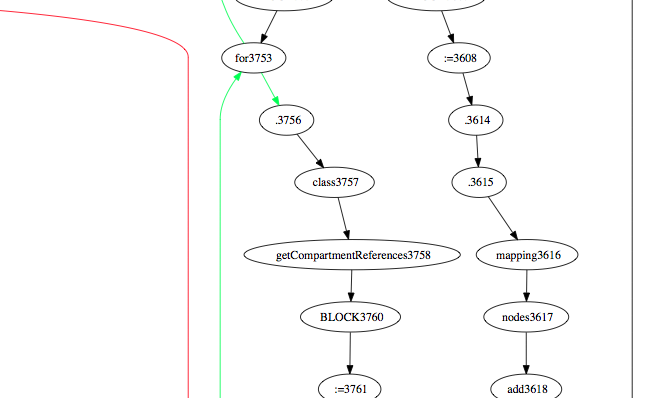
\includegraphics[scale=0.3]{figures/caseStudyProblem1}
\caption{The first problem with branch analysis of EuGENia}
\label{fig:caseStudyProblem1}
\end{figure}

The first problem was that when a conditional statement contained an operation call as part of the condition statement, this executing was causing the branch from the conditional statement to be marked as executed, regardless of whether the block of the conditional statement was actually being executed. An example of this is shown in Figure \ref{fig:caseStudyProblem1}. The for loop header contains the code \verb|class.getCompartmentReferences()| which is split into 3 vertices immediately following the for loop vertex. These are evaluated every time the for loop is reached, and if they return true then the for loop block is executed, and if not the loop is skipped. However, the branch execution listener code was noting that when any of the three vertices were executed that they satisfied the criteria:

\begin{enumerate}
\item The executed vertex is a child of the last executed vertex
\item The CFG of the executed vertex is a child of the CFG of the last executed vertex
\item The executed vertex is a valid type (i.e. whitelisted)
\end{enumerate}

With these conditions satisfied, the branch was being marked as having been executed. Two possible solutions were available. The first is to modify the AST to CFG conversion so that the vertices in the conditional statement are not executed. An attempt was made to implement this solution, but because of how the conversion algorithm deals with the case where there is no code following a loop block, it was not possible to do this `cleanly' (i.e. without lots of nasty conditional statements that would likely introduce bugs). Instead, the branch execution listener was modified so that the extra condition was included:

\begin{enumerate}
\setcounter{enumi}{3}
\item If the parent vertex is of type HELPERMETHOD then this vertex must be of type BLOCK
\end{enumerate}

The additional condition ensures that only the execution of a block under a conditional statement will cause the branch to be marked as executed.

\subsection{Operations}

Simple operation calls were covered during testing, and were thought to work correctly. However, while studying the output of branch analysis on the EuGENia source code, it was apparent that something was not working correctly as some branches were showing that no children had been executed, despite the fact that there definitely should have been at least one child executed (such as at an if .. else statement). An investigation of the cause showed that the problem was limited to when there was an operation call just prior to the problem conditional statement. In the branch execution listener there is a pointer to the last executed vertex that is used when calculating which branch has been executed. When an operation is called, the pointer will be updated within that operation. When control returns to the code that called the operation, the pointer will still be pointing to a vertex within the previously called operation. So when a branch is executed, the branch execution listener will decide that there is no connection between the last executed vertex pointer and the branch that has been executed, and not mark the branch as been executed as it should do.

To solve this problem, a stack was introduced. The idea was that when an operation call is executed the last executed vertex pointer is pushed to the stack, and when the operation call has completed, the stack is popped and stored in the last executed vertex pointer. The implementation was not quite as easy as it could have been. A function had to be implemented that determined whether an operation call had been executed by looking at the relative positions of the last executed vertex and the current executed vertex in the AST. The contents of the stack also have to be checked at each vertex execution because it seems that sometimes the execution listener doesn't always fire the end of an operation call vertex, and it can be necessary to pop more than one pointer from the stack on some occasions. 

\subsection{Path Coverage}

Unfortunately due to time constraints, and also the page limit of this report, I can not fully detail path coverage, and therefore I am counting it as not implemented for the purpose of evaluation and conclusion. In reality much of the work was done for path coverage, and what documentation was made will be included in the appendix.

\section{Results}

\subsection{Statement Coverage}

The results of the statement coverage are found in Appendix \ref{App:StatementCoverage}. The coverage of the existing test suite for EuGENia is 49\%. The output from the analysis clearly shows which section of the code have not been executed, and what needs to be tested in new test suites. For example, the for loop that `Processes EAttributes' (according to the comment above it) is never executed, and so none of the tests must contain models with EAttributes.

A lot of the non-executed statements are those in functions that were originally in the includes, Formatting.eol and ECoreUtil.eol. Despite the criticism of statement coverage that was outlined in the literature review, it is clear that it is sufficient for outlining some major gaps in the EuGENia test suite.

\subsection{Branch Coverage}

Out of 235 branches in EuGENia, 143 were executed (60.9\%). The graph that is produced is very large, too big to include as a whole graph. Instead the output code was modified to print operations as separate graphs so that they can be included more easily in Appendix. It is notable that the percentage of branches that were executed is higher than the percentage of overall statements that were covered. In a review of the statement coverage implementation it was noted that some statements are never marked as being executed, and so the percentage value is of less use that the highlighted syntax output.

% svn diff http://dev.eclipse.org/svnroot/modeling/org.eclipse.epsilon/trunk/plugins/org.eclipse.epsilon.eugenia/transformations/ECore2GMF.eol --revision 100:200 > output2.txt

\subsection{Requirements}

Earlier in the project a set of function and non-functional requirements were detailed. Each of these is now reviewed in Table \ref{tab:Functional}, with a discussion on if and how they have been satisfied.

\begin{table}[h]
    \begin{tabular}{|l|l|p{4.5in}|} \hline
    Requirement & Status        & Justification                                                                                                                                                                                   \\\hline
    F-01        & Satisfied     & It is possible to perform statement coverage on any EOL file with the statement coverage tool that has been implemented.                                                                        \\\hline
    F-02        & Satisfied     & The output HTML file contains the number of statements that have been executed.                                                                                                                 \\\hline
    F-03        & Satisfied     & The output HTML file highlights which statements have been executed, and does not highlight those that have not been executed.                                                                  \\\hline
    F-04        & Satisfied     & It is possible to perform branch coverage on any EOL file with the branch coverage tool that has been implemented.                                                                              \\\hline
    F-05        & Satisfied     & The output from the branch coverage analysis contains a text file that states the number of branches that have been executed.                                                                   \\\hline
    F-06        & Satisfied     & The generated control flow graph highlights branches that have been executed in green, and those that have not are highlighted in red.                                                          \\\hline
    F-07        & Not Satisfied & The user cannot perform path coverage on any EOL file because time limitations prevented this from being completed. However, the majority of the work has been done to implement path coverage. \\\hline
    F-08        & Not Satisfied & Because the user cannot perform path coverage, the number of executed paths cannot be determined.                                                                                               \\\hline
    F-09        & Not Satisfied & Because the user cannot perform path coverage, the user cannot see which paths were executed, and which were not.                                                                               \\\hline
    \end{tabular}
    \caption{Evaluation of functional requirements}
    \label{tab:Functional}
\end{table}

With the non-functional requirements it is a little more difficult to say for sure whether they have been satisfied or not. There were two core requirements, repeated for each of the three coverage types. The first core requirement was that the coverage analysis will not take an `excessive' amount of time to complete. What is excessive can only be decided by the user. In my experience, the tools that were investigated during the literature review did not add more than 5 seconds to the overall execution time of a test suite.

%Baseline: 56.9, 52.4, 53.6
%Statement: 62.9, 63.2, 62.3
%Branch: 68.4, 65.9, 65.7

The execution time of the EuGENia test suite was recorded with no coverage analysis enabled, with statement coverage enabled, and finally with branch coverage enabled. Each test was run three times, with the average and standard deviation recorded. The results are shown in Table \ref{tab:runTimes}.

\begin{table}[h]
\centering
    \begin{tabular}{|p{1in} | p{0.6in} |p{0.6in} |p{0.6in} |p{0.6in} |p{0.8in} |} \hline
    Coverage Type & Time 1 (seconds) & Time 2 (seconds) & Time 3 (seconds) & Average Time (seconds) & Standard Deviation (seconds) \\\hline
    None          & 56.9             & 52.4             & 53.6             & 54.3                   & 2.3                          \\\hline
    Statement     & 62.9             & 63.2             & 62.3             & 62.8                   & 0.5                          \\\hline
    Branch        & 68.4             & 65.9             & 65.7             & 66.7                   & 1.5                          \\\hline
    \end{tabular}
    \caption{Run Times of the EuGENia test suite}
    \label{tab:runTimes}
\end{table}

It is interesting to note that both statement and branch coverage increase the run time quite significantly (15\% and 23\%, respectively). A more careful analysis showed that the slowdown was not in the analysis and output of the statistics, but in the execution listener code. I find it to be surprising that the statement coverage code slows the execution down by such a lot, because the execution listener really does not do a great deal. More detailed profiling is required to understand why this is the case. It may be that some inefficient code can be changed to speed up the listener.

On the other hand, the speed of the branch analysis does not come as a surprise. As each statement is executed, a partial traversal of the AST is performed to determine if the executed statement is in the same operation as the previously executed statement, and this will cause a slowdown.

%While it is purely subjective, I am going to say that the core requirements for statement and branch coverage have been satisfied. I will discuss possible further work to speed up the code in the next chapter. Because path coverage has not been completely implemented, I am counting the related core non-functional requirements as not satisfied.

Through extensive testing of small programs, and the case study that was detailed in this chapter, I can conclude that the core requirements for statement and branch coverage have been satisfied.

The conversion algorithm provides an interface for new statements to be included in the conversion, making the framework easily extensible. For the other components of the framework, I can not think of a reason why they would need modification to work with other languages, as none have any EOL specific dependencies, and so the requirement is satisfied.

Finally, there was requirement that the output is simple to understand. For statement coverage I have followed what was commonly seen in other coverage tools. With branch coverage, the graph that is output clearly shows which branches have been executed, and which have not, and I am happy that the requirement has been satisfied.
\chapter{Conclusions}

% Further work:

% * fallthrough switch statements
% * proper path analysis on loops

\bibliography{bibliography}

\addcontentsline{toc}{chapter}{Appendices}
\addtocontents{toc}{\protect\setcounter{tocdepth}{-1}}
\appendix

%\newpage
\chapter{\\The AST to CFG class}
\label{App:SampleEuGENia}
%
\lstinputlisting[language=EOL]{code/sample_gmf.emf}
%
%\lstinputlisting[language=java, breaklines=true]{/Users/thomaswormald/Documents/workspace/all/org.eclipse.epsilon/trunk/plugins/org.eclipse.epsilon.eol.engine/src/org/eclipse/epsilon/eol/parse/ASTtoCFG.java}
%
%%\newpage
%%\chapter{\\Statement Coverage HTML Output Class}
%%\label{App:StatementHTMLOutput}
%%\lstinputlisting[language=java]{code/StatementCoverageToHTML.java}


\end{document}
